% --------------------------------------------------------------------------- %
% --------------------------------------------------------------------------- %
\chapter{Missing Transverse Momentum}
\label{ch:MET}
% --------------------------------------------------------------------------- %
% --------------------------------------------------------------------------- %
In the final state targeted by this analysis, a gravitino is proposed as the LSP.
This particle is weakly interacting and makes a good dark matter candidate
which lead to signal events having large values of \MET\ due to this particle escaping detection.
It is important that \MET\ from standard model processes is predicted accurately.
\MET\ can be calculated using the full collection of PF candidates described in section~\ref{subs:particleflow}.
In the following sections, \MET\ calculations and corrections are described in detail.

\section{raw \texorpdfstring{\MET}{MET}}

Calculating \MET\ using PF candidates is done by summing the transverse momentum vectors of all the PF candidates, described in equation~\ref{eqn:rawmet}.

\begin{equation}
  \label{eqn:rawmet}
\mathrm{\overrightarrow{E_{T}^{miss}} = -\sum_{i}\overrightarrow{p}_{T}^{i}}
\end{equation}

When \MET\ is calculated without any calibration applied to the pf candidates, it is known as raw MET.

\subsection{Sources of \texorpdfstring{\MET}{MET}}
\label{sec:metsources}
\MET\ comes from three main sources,
noise in the detector from various sources,
resolution effects due to mismeasurement of physics objects and
visible particles from the hard interaction being too far forward in $\eta$ to be within the detector geometry (referred to as fake \MET)
and particles from real physics processes not interacting with the detector thereby escaping detection.

\MET\ due to noise in the detector can lead to huge tails in the \MET\ distribution.
The size of this effect is shown in figure~\ref{fig:cleanmet} for the data taken in 2012.
A set of filters is applied to mitigate these effects,
and the details of these filters is described in section~\ref{ssec:metfilter}.

\begin{figure}[!ht]
  \begin{center}
    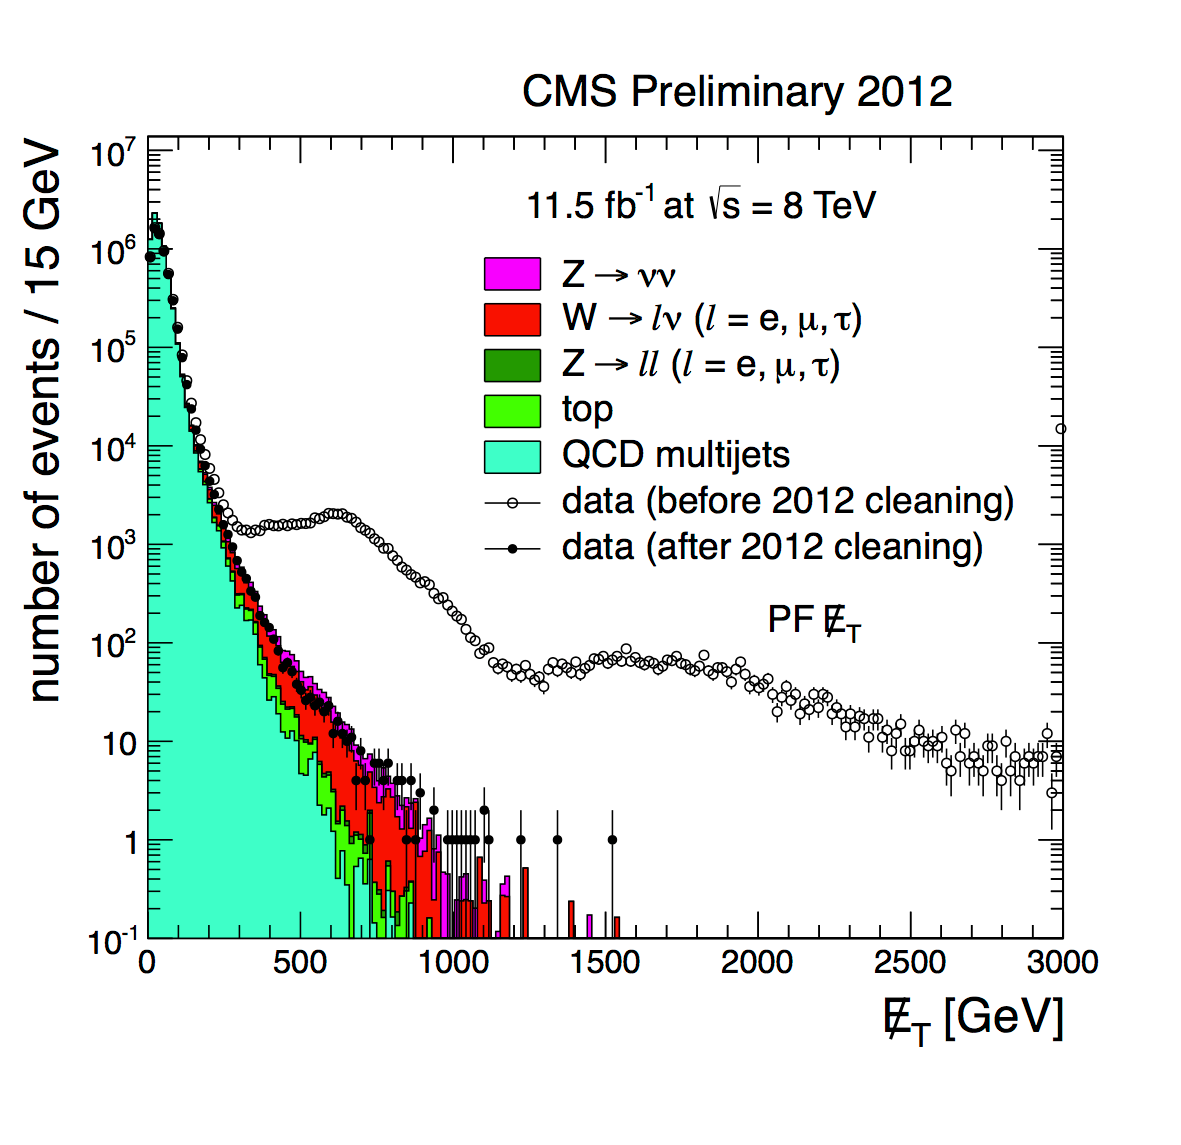
\includegraphics[width=0.8\textwidth]{MET/figs/Fig4EventCleaning.pdf}
    \caption{
      \label{fig:cleanmet}
      \MET\ distributions for events passing the dijet selection without 2012 cleaning algorithms applied (open markers),
      with 2012 cleaning algorithms applied including the one based on jet identification requirements (filled markers),
      and events from MC (filled histograms).
    }
  \end{center}
\end{figure}

Particles that do not interact with the detector that lead to real \MET\ can be standard model neutrinos, or particles from BSM theories such as the $\mathrm{\tilde{G}}$.
Since this analysis is searching in regions with large \MET, it is very important to be able to identify and measure backgrounds with fake \MET and real \MET.

\section{Type-1 \texorpdfstring{\MET}{MET}}
\label{sec:t1met}
In order to reconstruct \MET\ with high precision, corrections that are made to physics objects need to be propagated to the \MET\ variable.
The corrections with the largest impact on the \MET\ resolution are the jet corrections, since jets have the worst resolution.
Energy from pileup in each event is deposited randomly in the detector, and is expected to be balanced.
It can happen that some pileup energy deposited overlaps with energy from a jet coming from the hard interaction.
A correction is applied to the jet to account for this effect,
however if the pileup energy removed from each jet's cone were to be propagated to the \MET, it would create an imbalance.
This is taken care of by adding the pileup energy back in, and the overall correction to \MET\ is called the Type 1 correction.

Type 1 \MET\ refers to a version of \MET\ where the corrections that are applied to jets are propagated to the \MET\ calculation as described in section~\ref{ssec:jets}.
The correction factors applied to the jets are derived for jets down to 10 \gev.
The way these corrections are propagated to the \MET\ is not as straightforward as just adding the corrections vectorially with the \MET.

The jets we use in this analysis are made using all the pf candidates, except the charged pf candidates that are not associated with the primary vertex.
Leptons and photons are included in the collection of pf candidates used when clustering jets.
The jet corrections are meant to correct jets that come from hadronic objects, such as quarks and gluons.
If the jet corrections are applied to lepton and photon objects, the
The jet corrections are not meant to be applied to lepton and photon objects.
When propagating the jet corrections to the \MET, we exclude corrections on jets with an electromagnetic fraction larger than 90\%,
and remove the pf muon candidates from the jet when deriving the corrections.
This effectively removes photons and leptons from the objects that get corrected.

\subsection{Data vs. MC Comparison}
\label{subs:MET_datavsmc}
It is important to understand how well \MET\ is simulated in MC in order to validate the MC samples used to simulate signal and certain background predictions.
Studies were done to check the agreement in data vs. MC in different detector subsystems.
The studied region is defined simply by having at least two leptons coming from a Z boson, so no real \MET\ is expected in these events.
The \MET\ components are studied separately in different detector subsystems by choosing several categories of pf candidate type and $\eta$ region defined in table~\ref{tab:subdetector_eta}.
Charged candidates in the region with $\eta < 2.4$, can be used to study the tracker,
neutral hadronic candidates can be used to study the HCAL,
and neutral electromagnetic candidates can be used to study the ECAL.
The \MET in each region is defined by calculating the negative magnitude of the vector-sum of only the charged, neutral hadronic, or neutral electromagnetic PF candidates.
The plots showing the agreement for each \MET\ component are shown in figures~\ref{fig:chpfcands},~\ref{fig:phpfcands}, and~\ref{fig:nupfcands} respectively. 
The charged  component of \MET\ shows reasonable agreement over the entire CMS detector.
The neutral electromagnetic component of \MET\ shows good agreement in the tracker volume of CMS, and the agreement is bad for cadidates outside of the tracker.
The neutral hadronic component of \MET\ shows poor agreement in the tracker volume of CMS, and the agreement gets much worse for cadidates in the very forward region.

\begin{table}[htb]
\scriptsize
\begin{center}
\caption{
Definitions for the $\eta$ region chosen to define each subdetector region are listed in this table.
\label{tab:subdetector_eta}}
\begin{tabular}{l|c}

\hline
Subdetector Region     & $\eta$ cut \\
\hline
Barrel                 & $|\eta| < 1.3$ \\
Transition region      & $1.3 < |\eta| < 1.6$ \\
Endcap with tracker    & $1.6 < |\eta| < 2.4$ \\
Endcap without tracker & $2.4 < |\eta| < 3.0$ \\
HF region              & $|\eta| > 3.0$ \\
\hline
\end{tabular}
\end{center}
\end{table}


\begin{figure}[!ht]
\begin{center}
\begin{tabular}{cc}
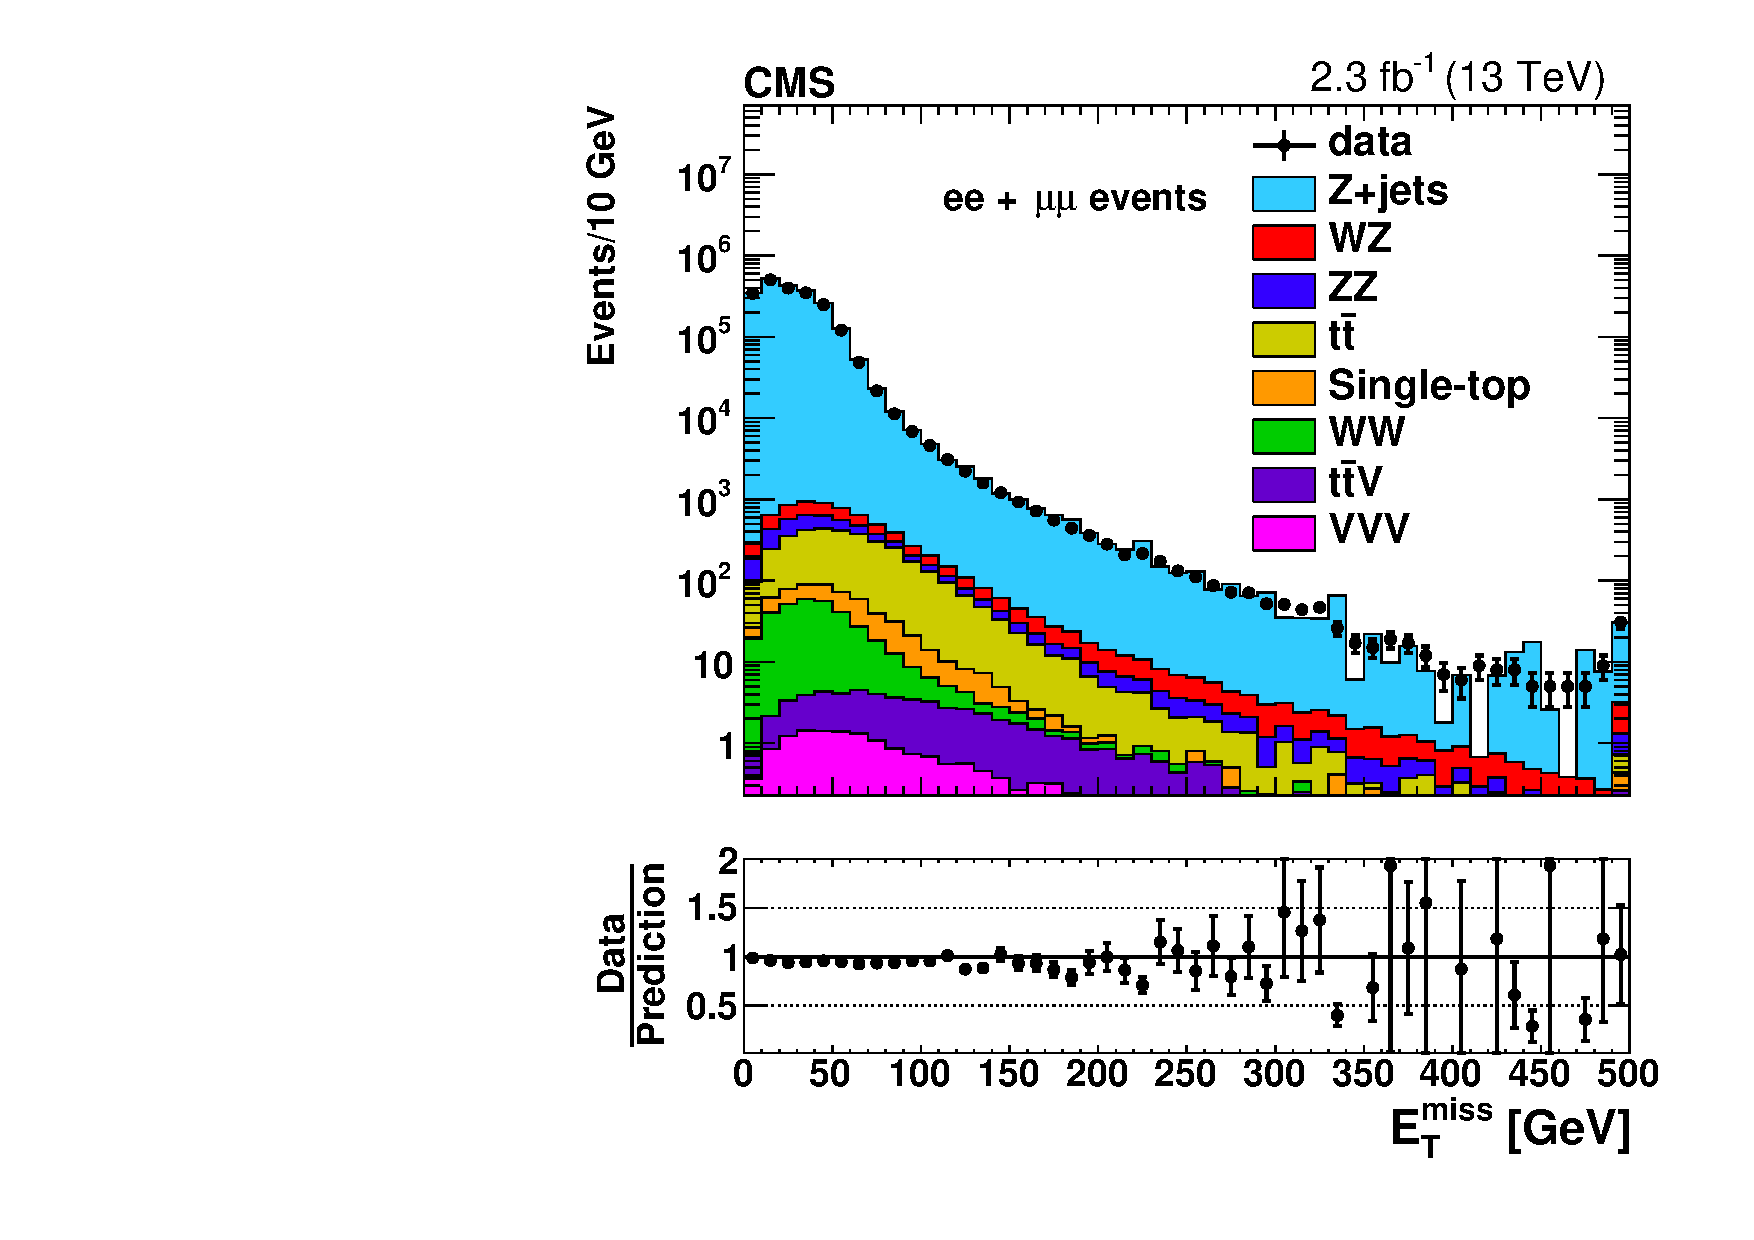
\includegraphics[width=0.4\textwidth]{MET/figs/h_met_chpfcands_0013_pt_ll_signalregion_inclusive_passtrig.pdf} &
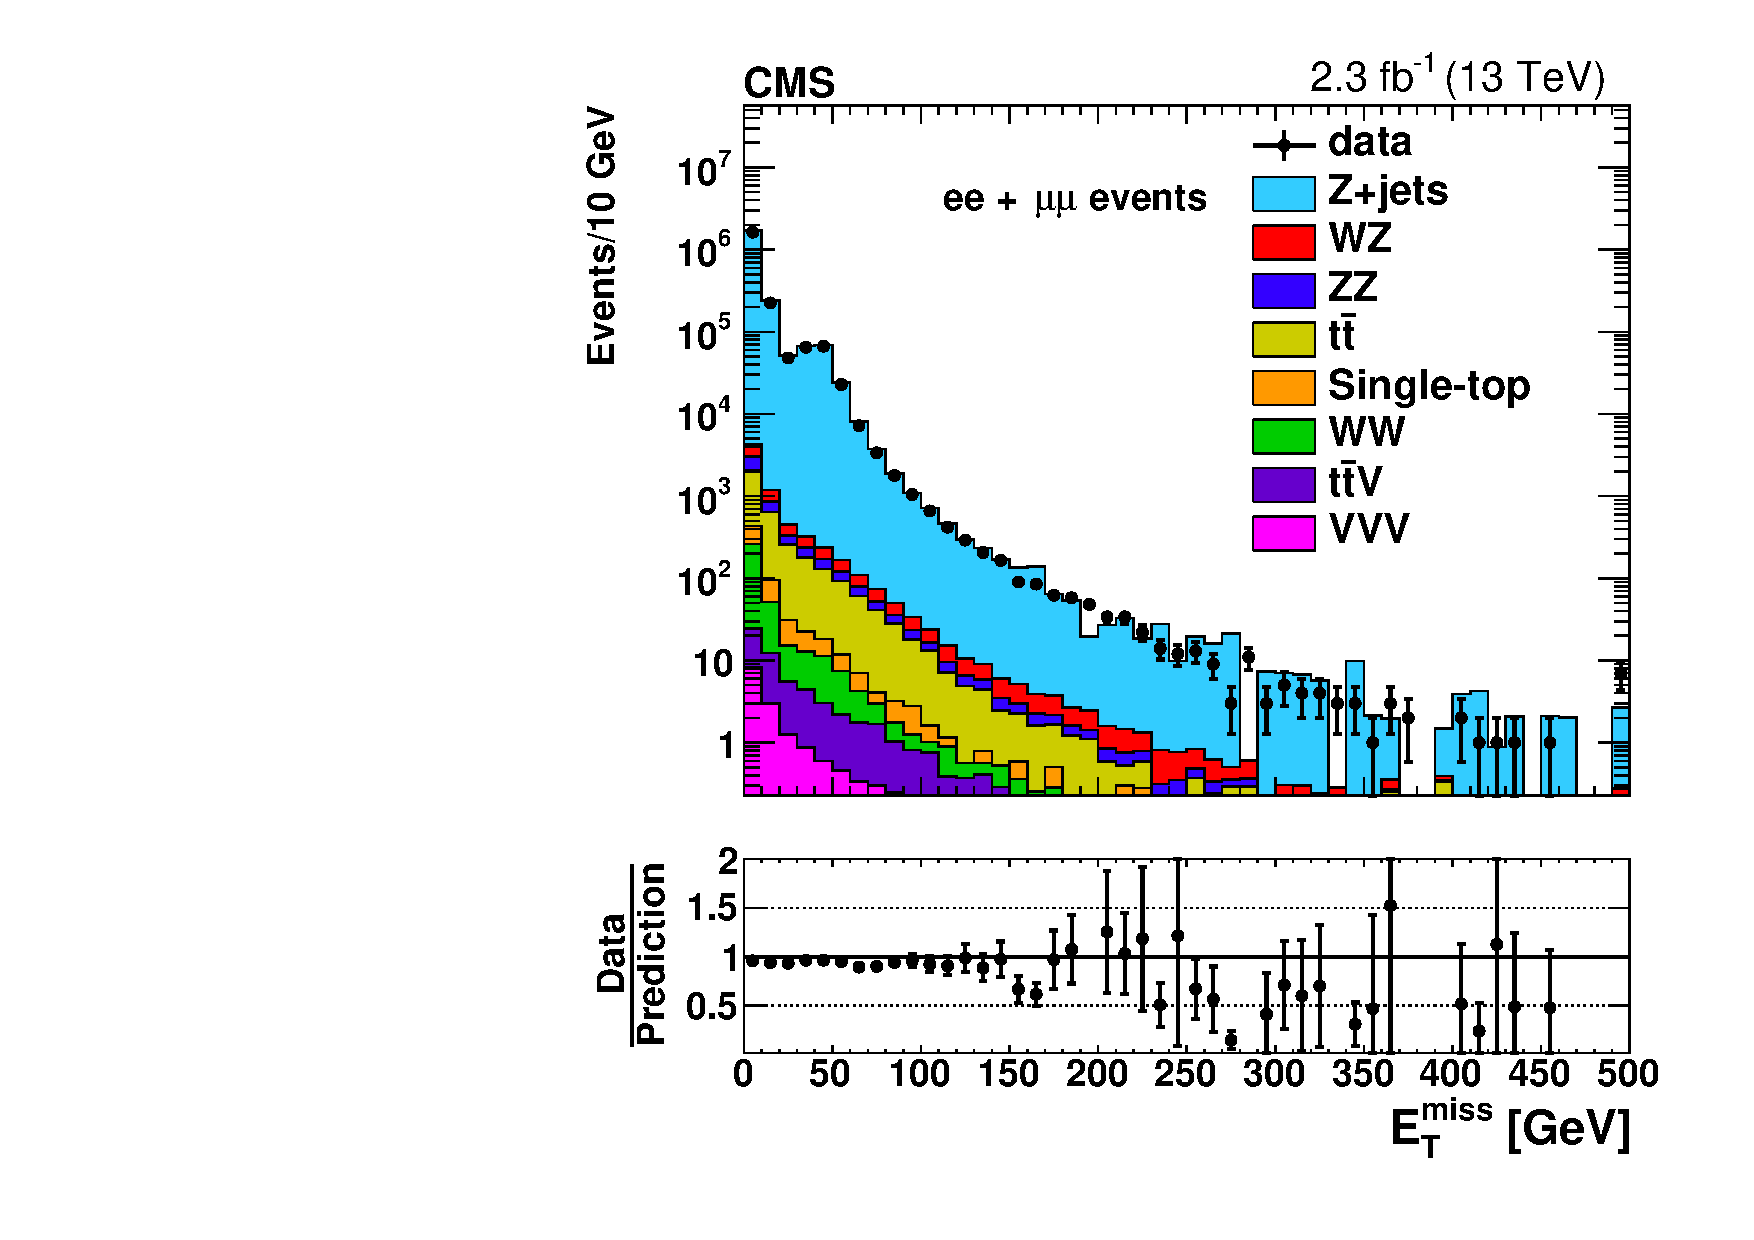
\includegraphics[width=0.4\textwidth]{MET/figs/h_met_chpfcands_1316_pt_ll_signalregion_inclusive_passtrig.pdf} \\
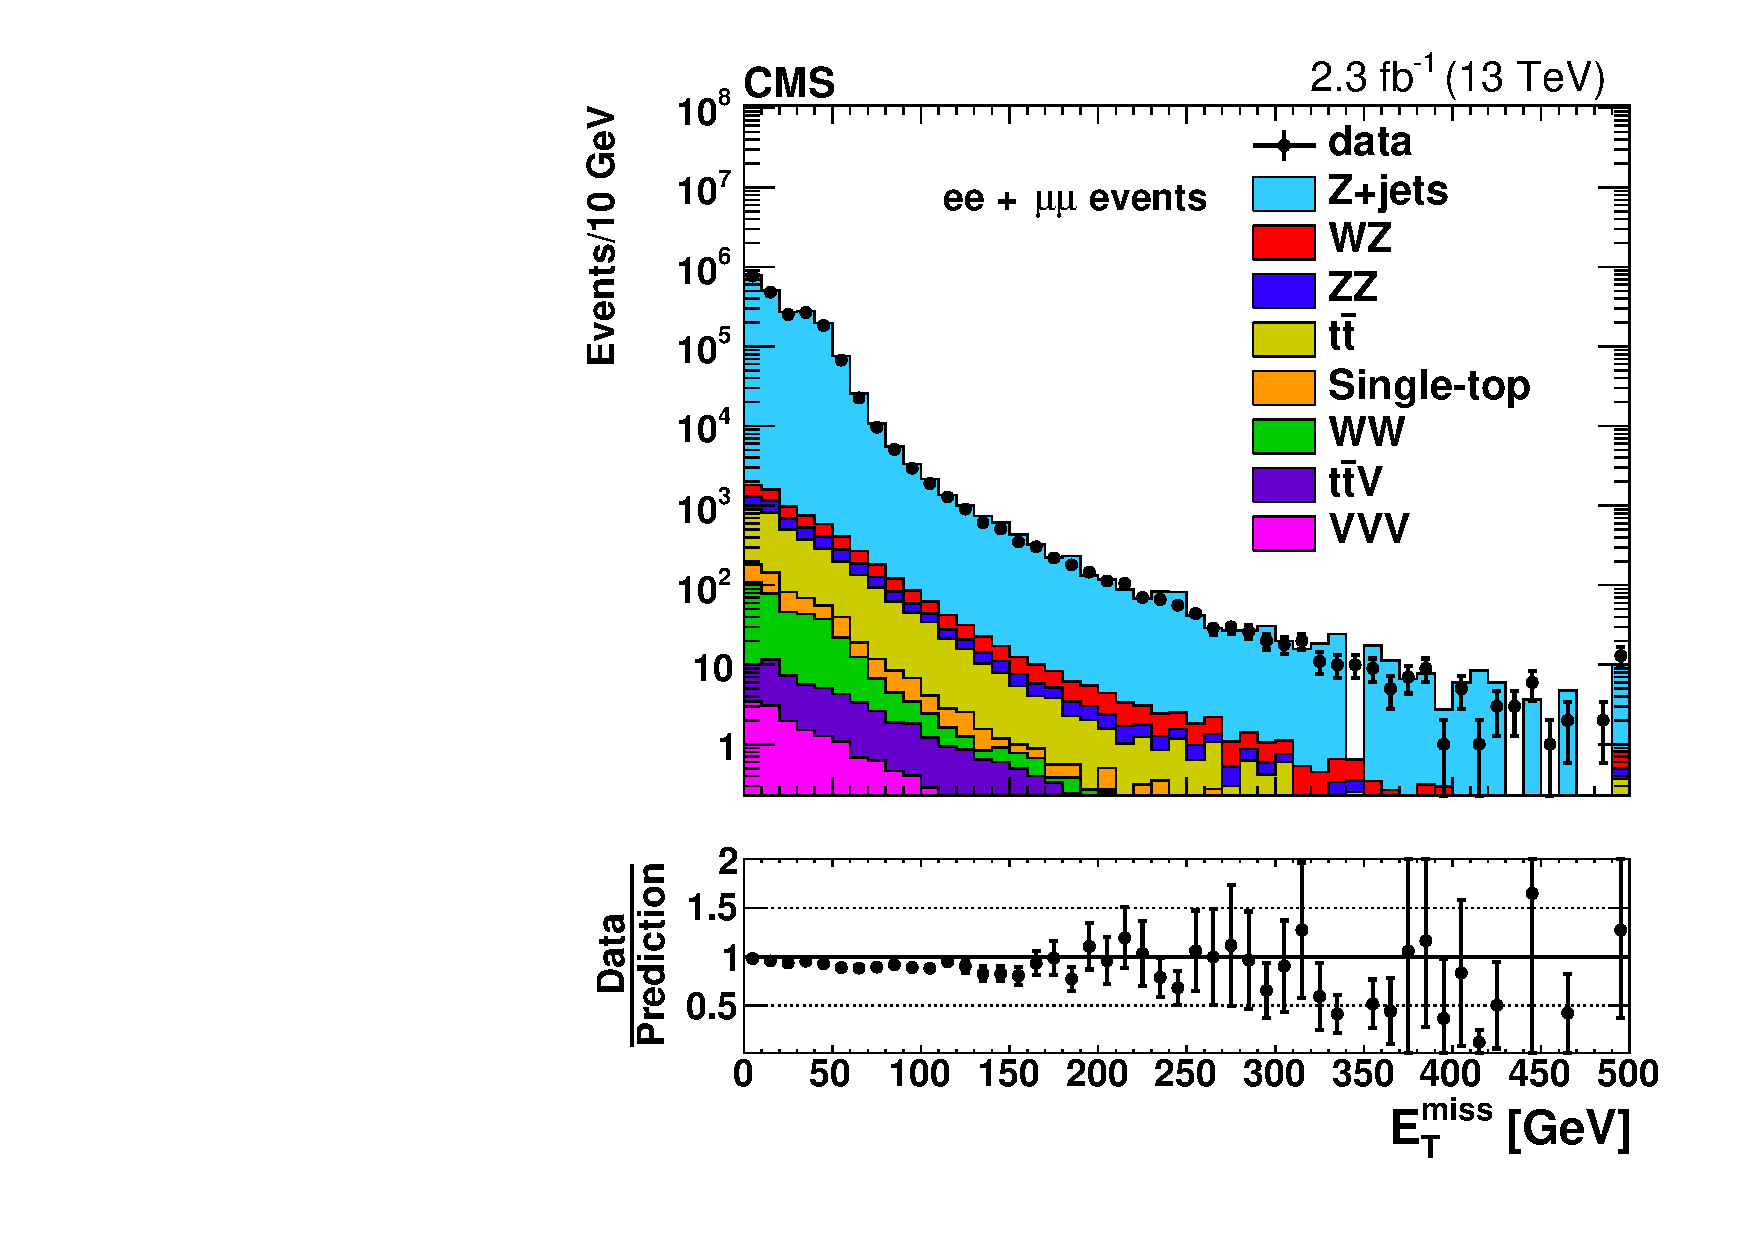
\includegraphics[width=0.4\textwidth]{MET/figs/h_met_chpfcands_1624_pt_ll_signalregion_inclusive_passtrig.pdf} &
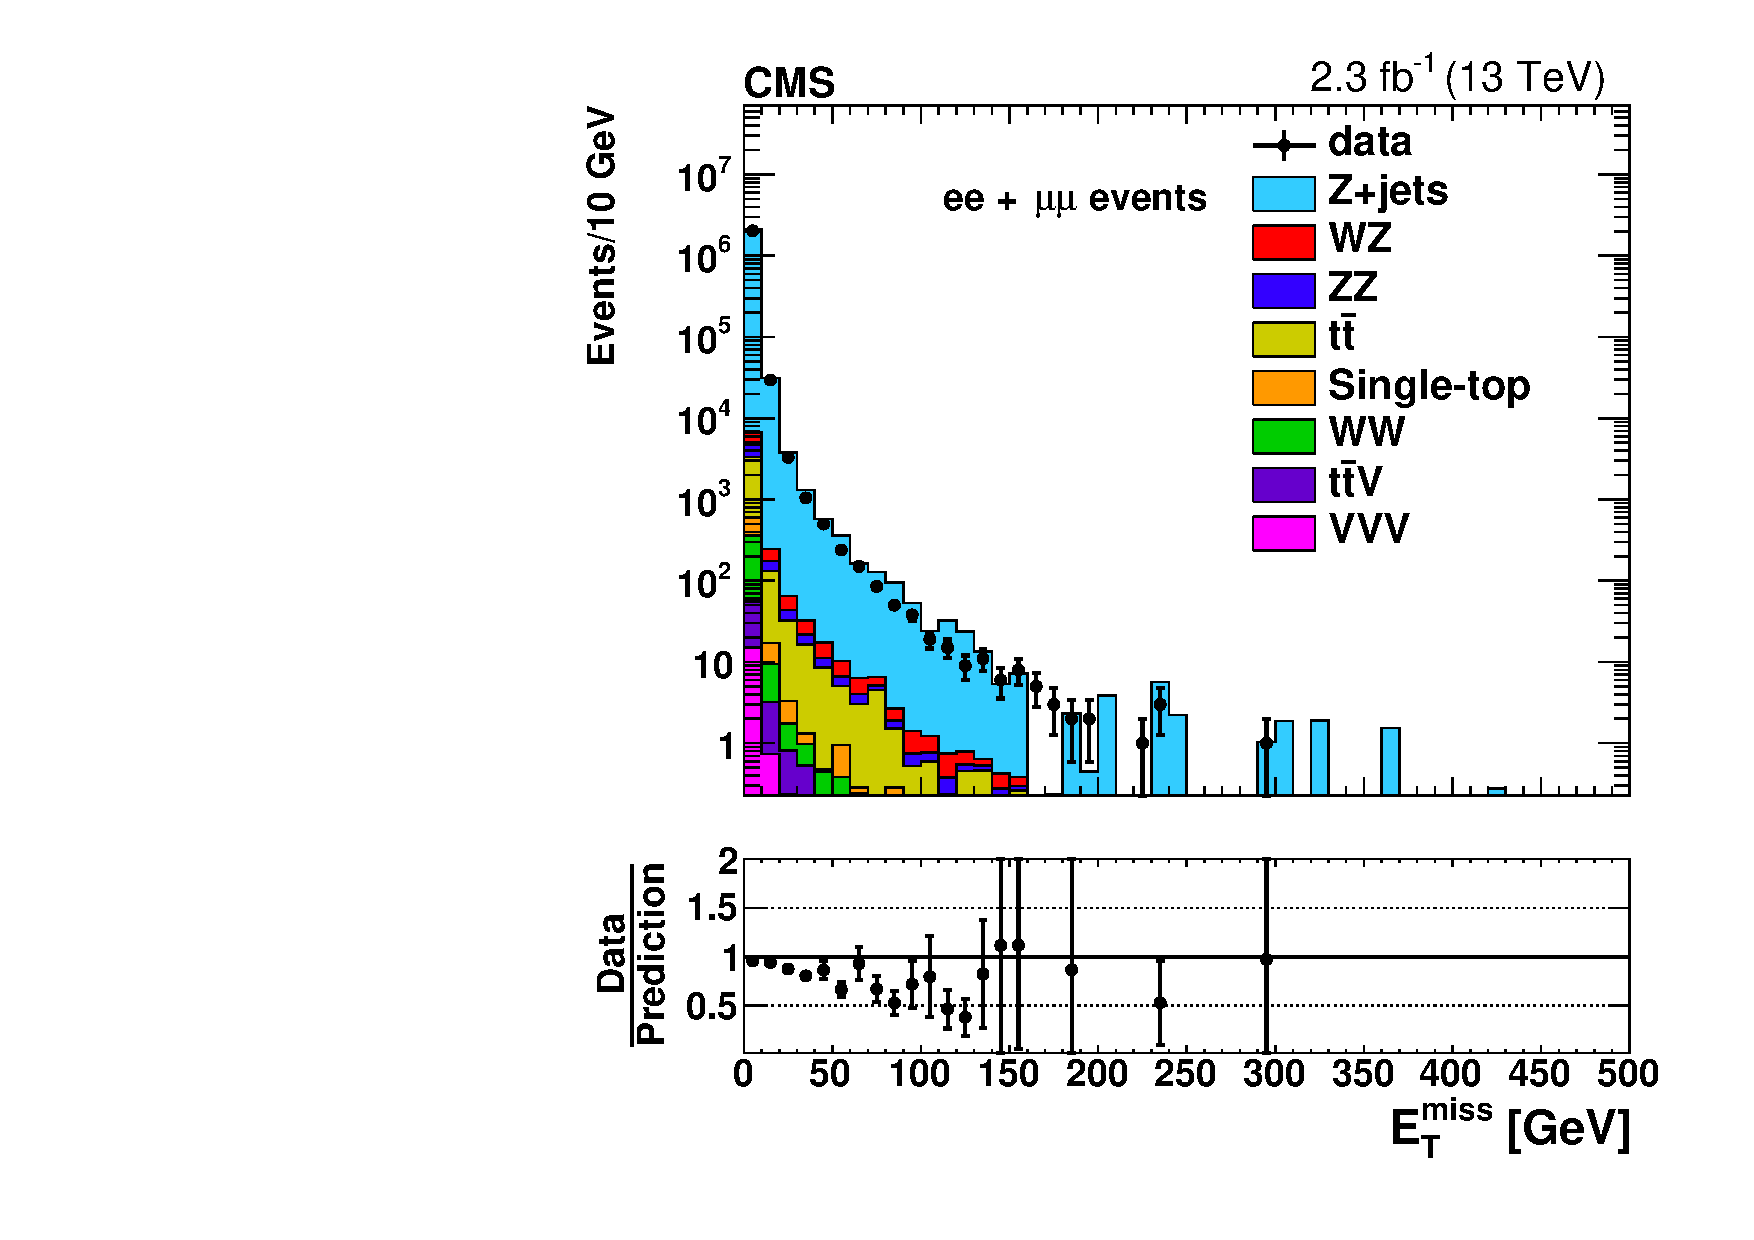
\includegraphics[width=0.4\textwidth]{MET/figs/h_met_chpfcands_2430_pt_ll_signalregion_inclusive_passtrig.pdf} \\
\end{tabular}
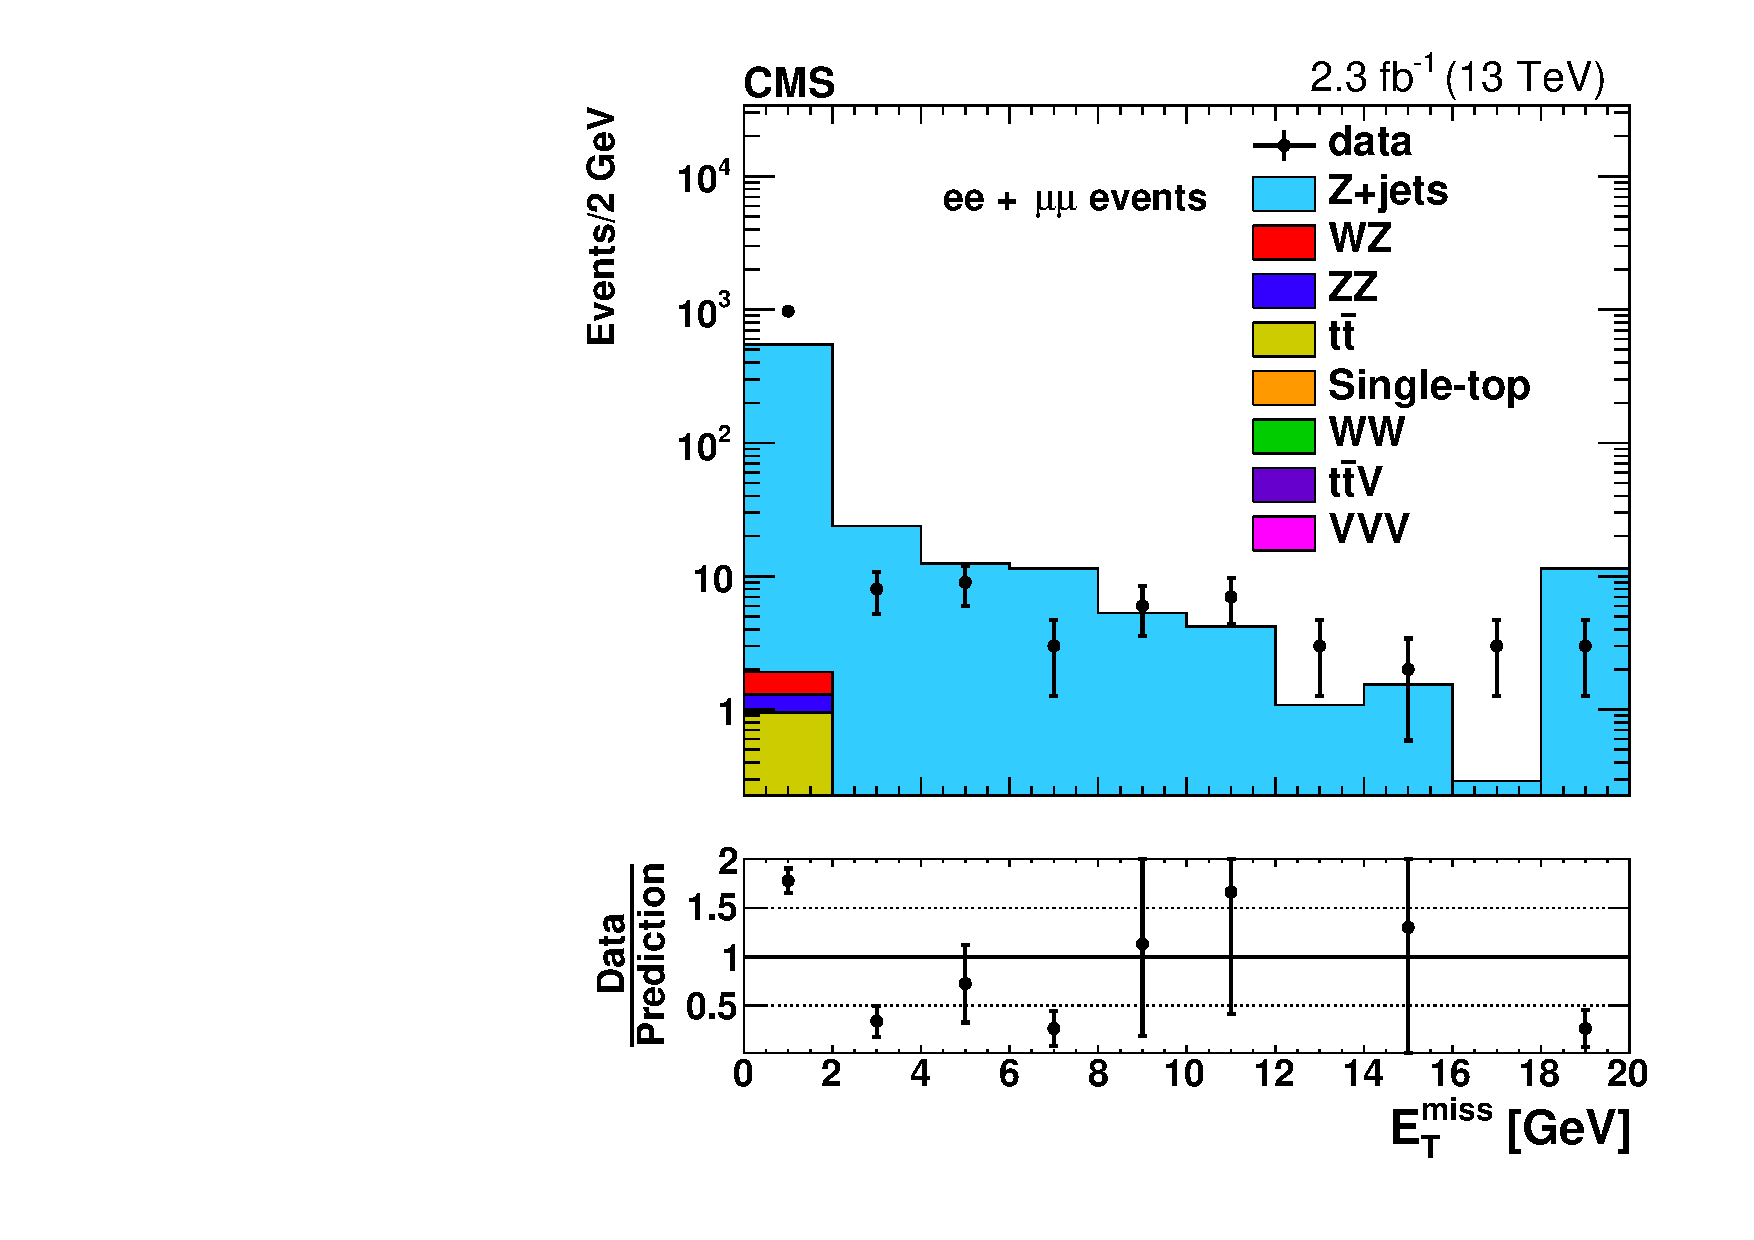
\includegraphics[width=0.4\textwidth]{MET/figs/h_met_chpfcands_30in_pt_ll_signalregion_inclusive_passtrig.pdf} 
\caption{The \MET\ distribution is shown for charged PF candidates only.
The top row shows the barrel region on the left and transition region between the barrel and endcap on the right,
the second row shows the endcap region including the tracker on the left and endcap region excluding the tracker on the right
and the bottom row shows the HF region only.
\label{fig:chpfcands}
}
\end{center}
\end{figure}

\begin{figure}[!ht]
  \begin{center}
    \begin{tabular}{cc}
      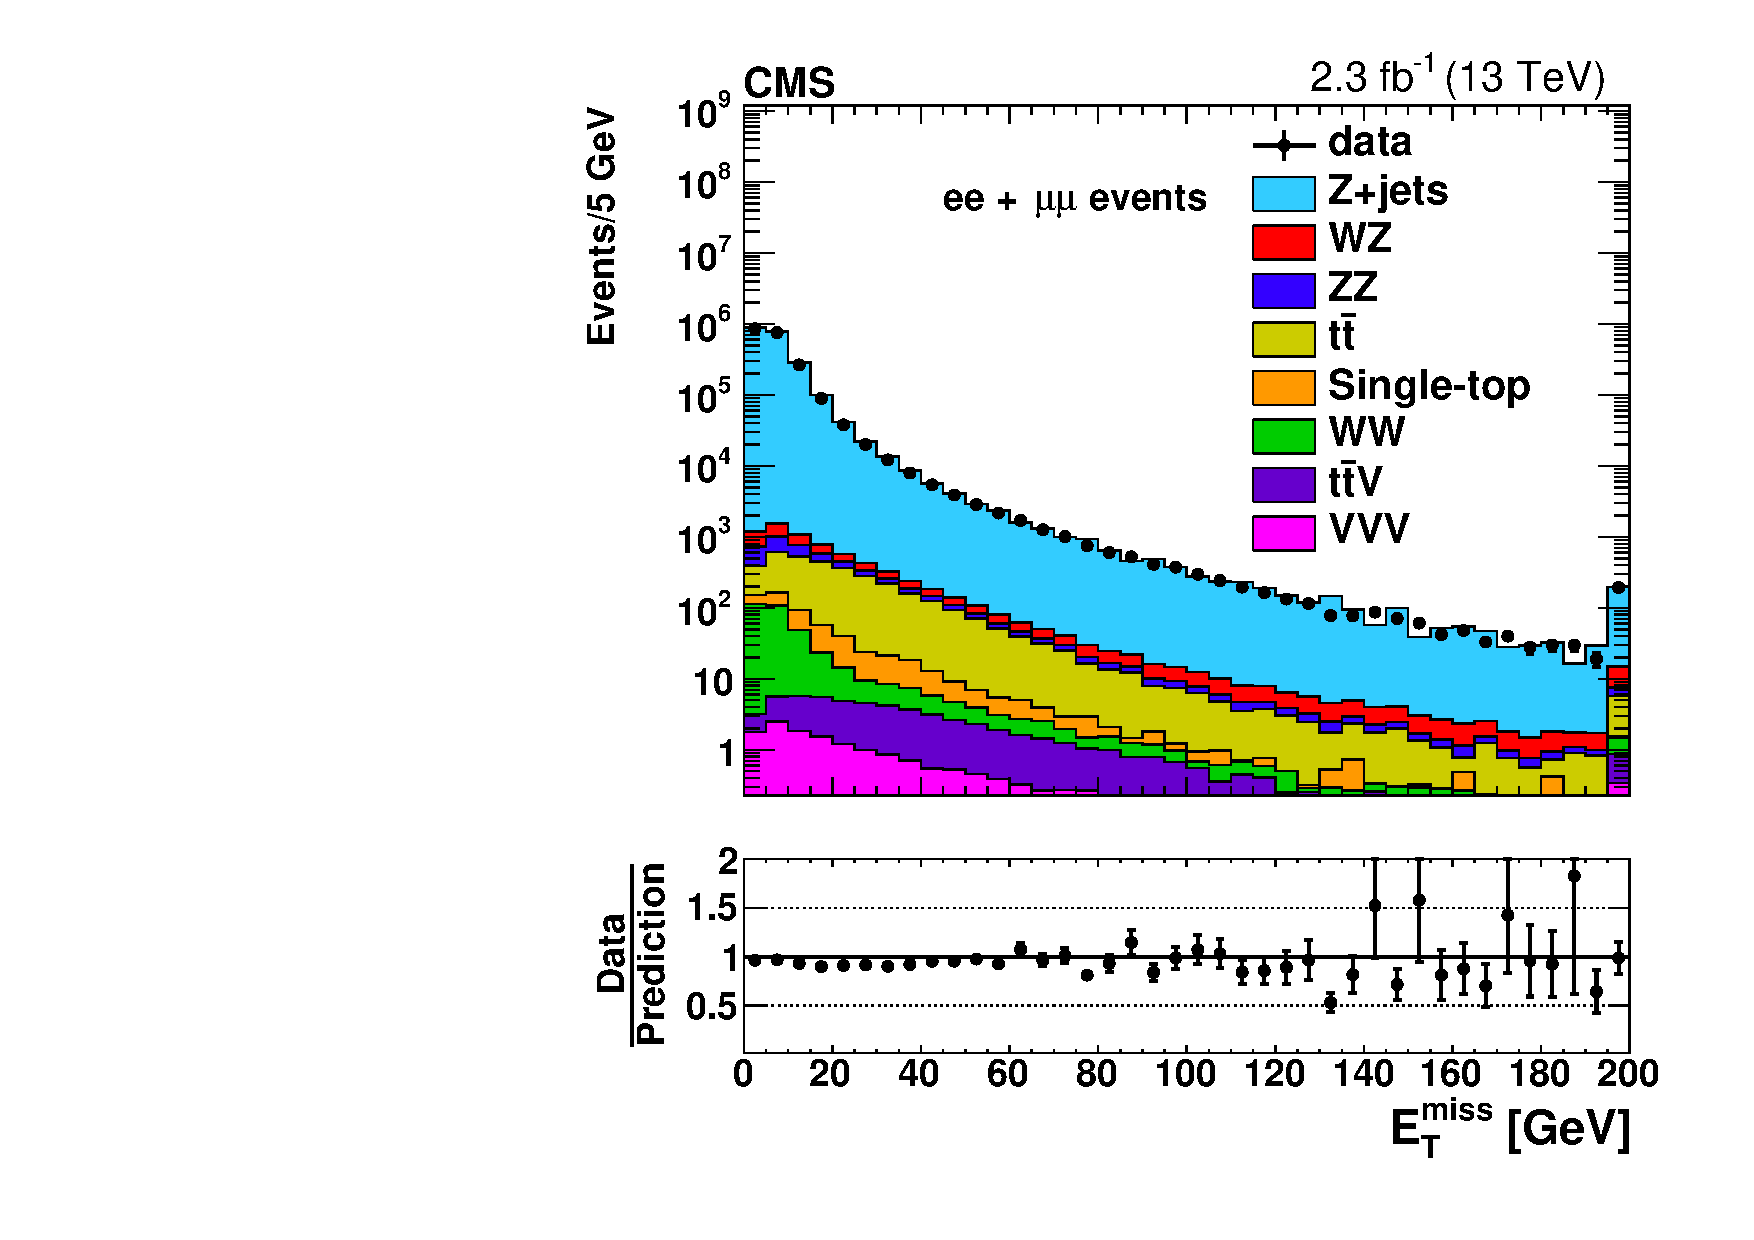
\includegraphics[width=0.4\textwidth]{MET/figs/h_met_phpfcands_0013_pt_ll_signalregion_inclusive_passtrig.pdf} &
      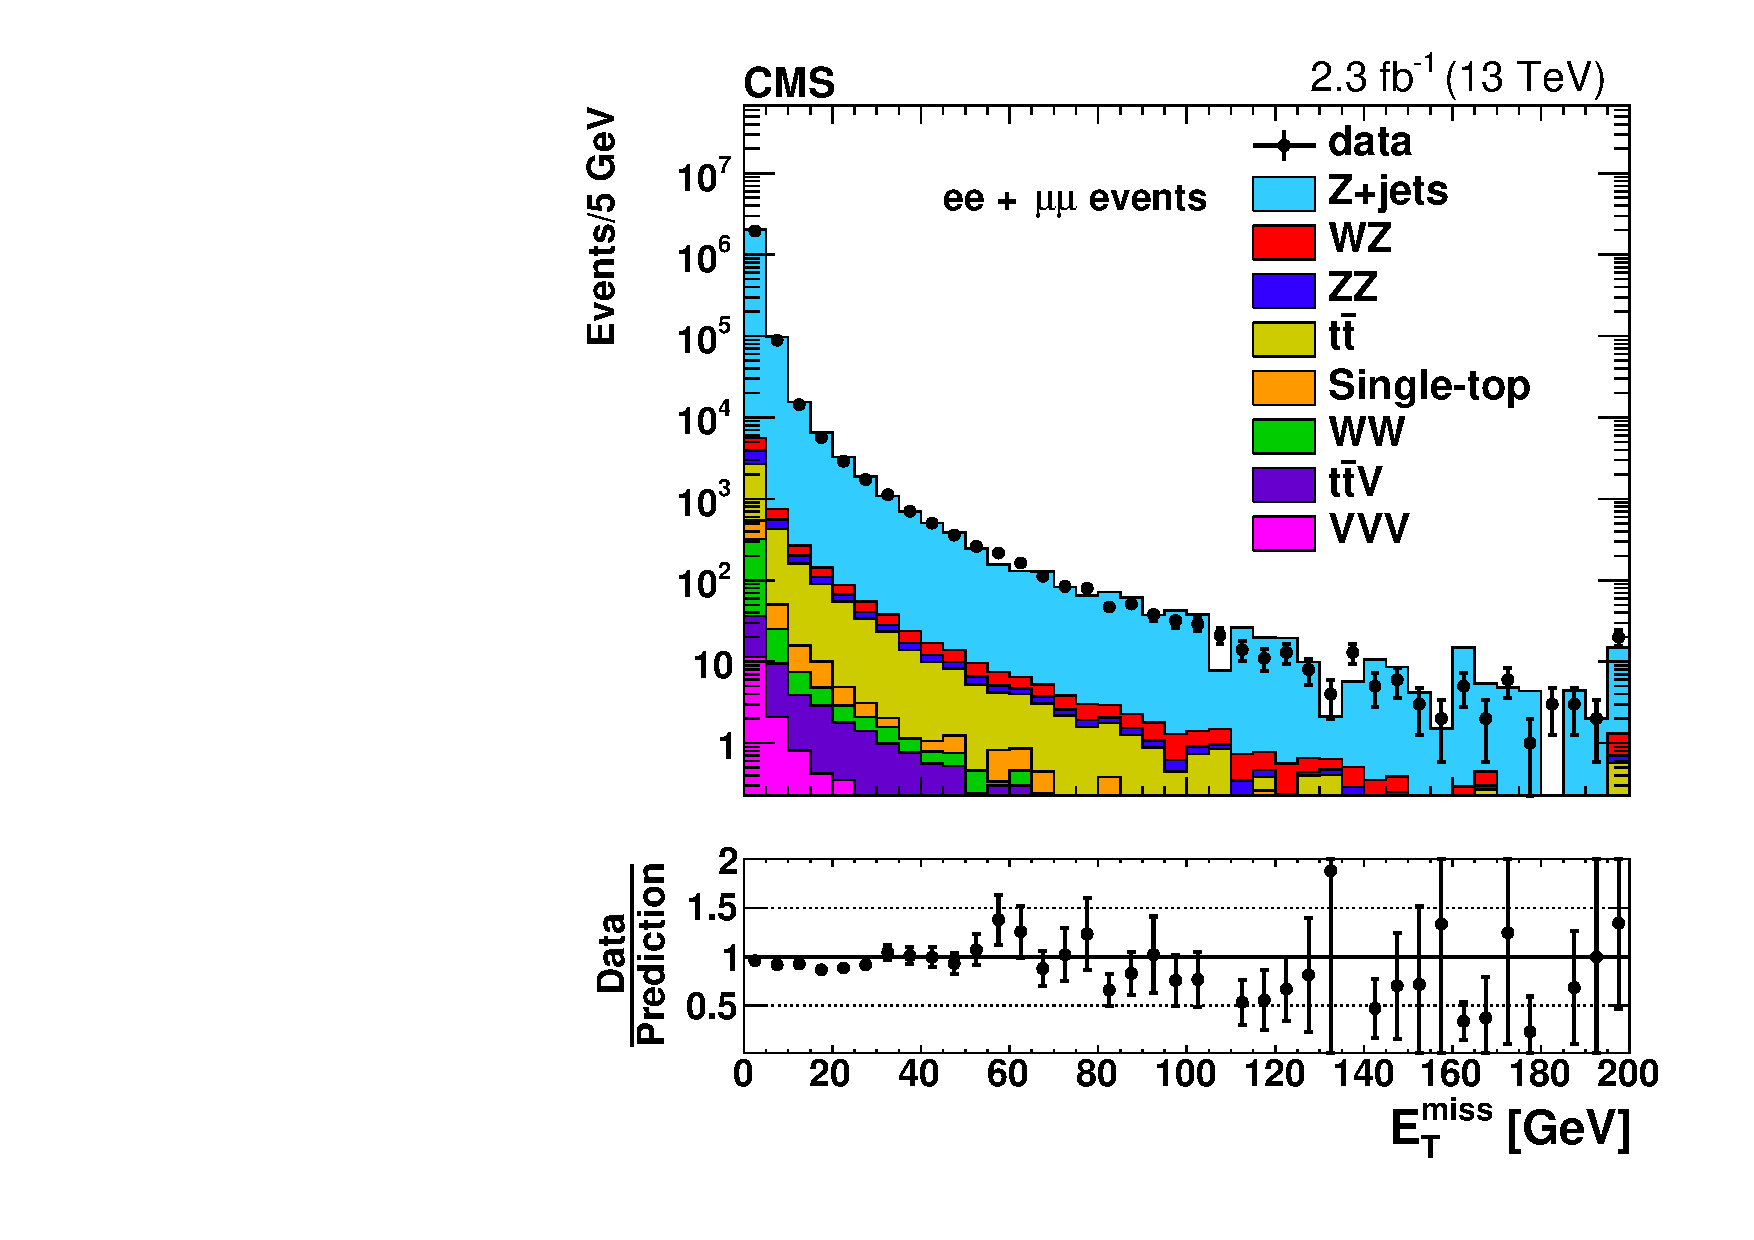
\includegraphics[width=0.4\textwidth]{MET/figs/h_met_phpfcands_1316_pt_ll_signalregion_inclusive_passtrig.pdf} \\
      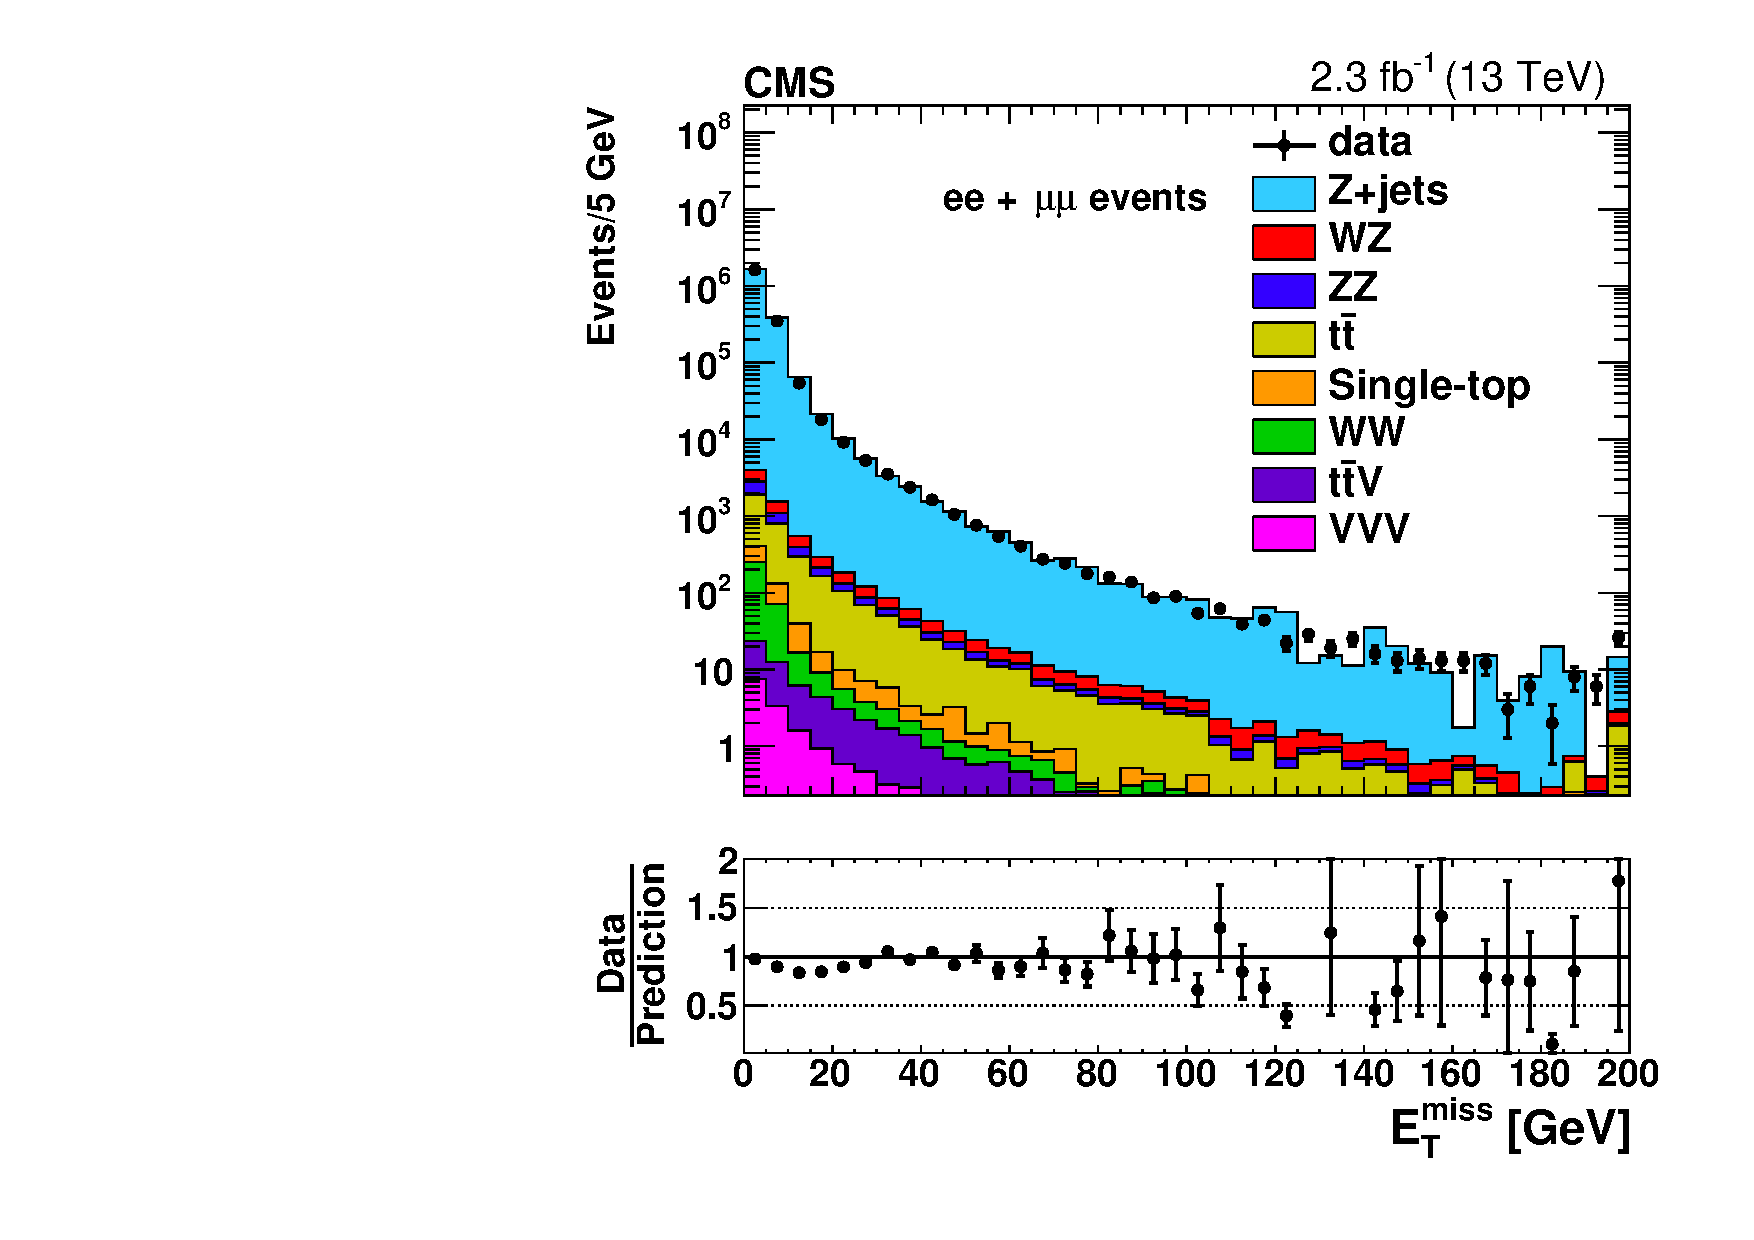
\includegraphics[width=0.4\textwidth]{MET/figs/h_met_phpfcands_1624_pt_ll_signalregion_inclusive_passtrig.pdf} &
      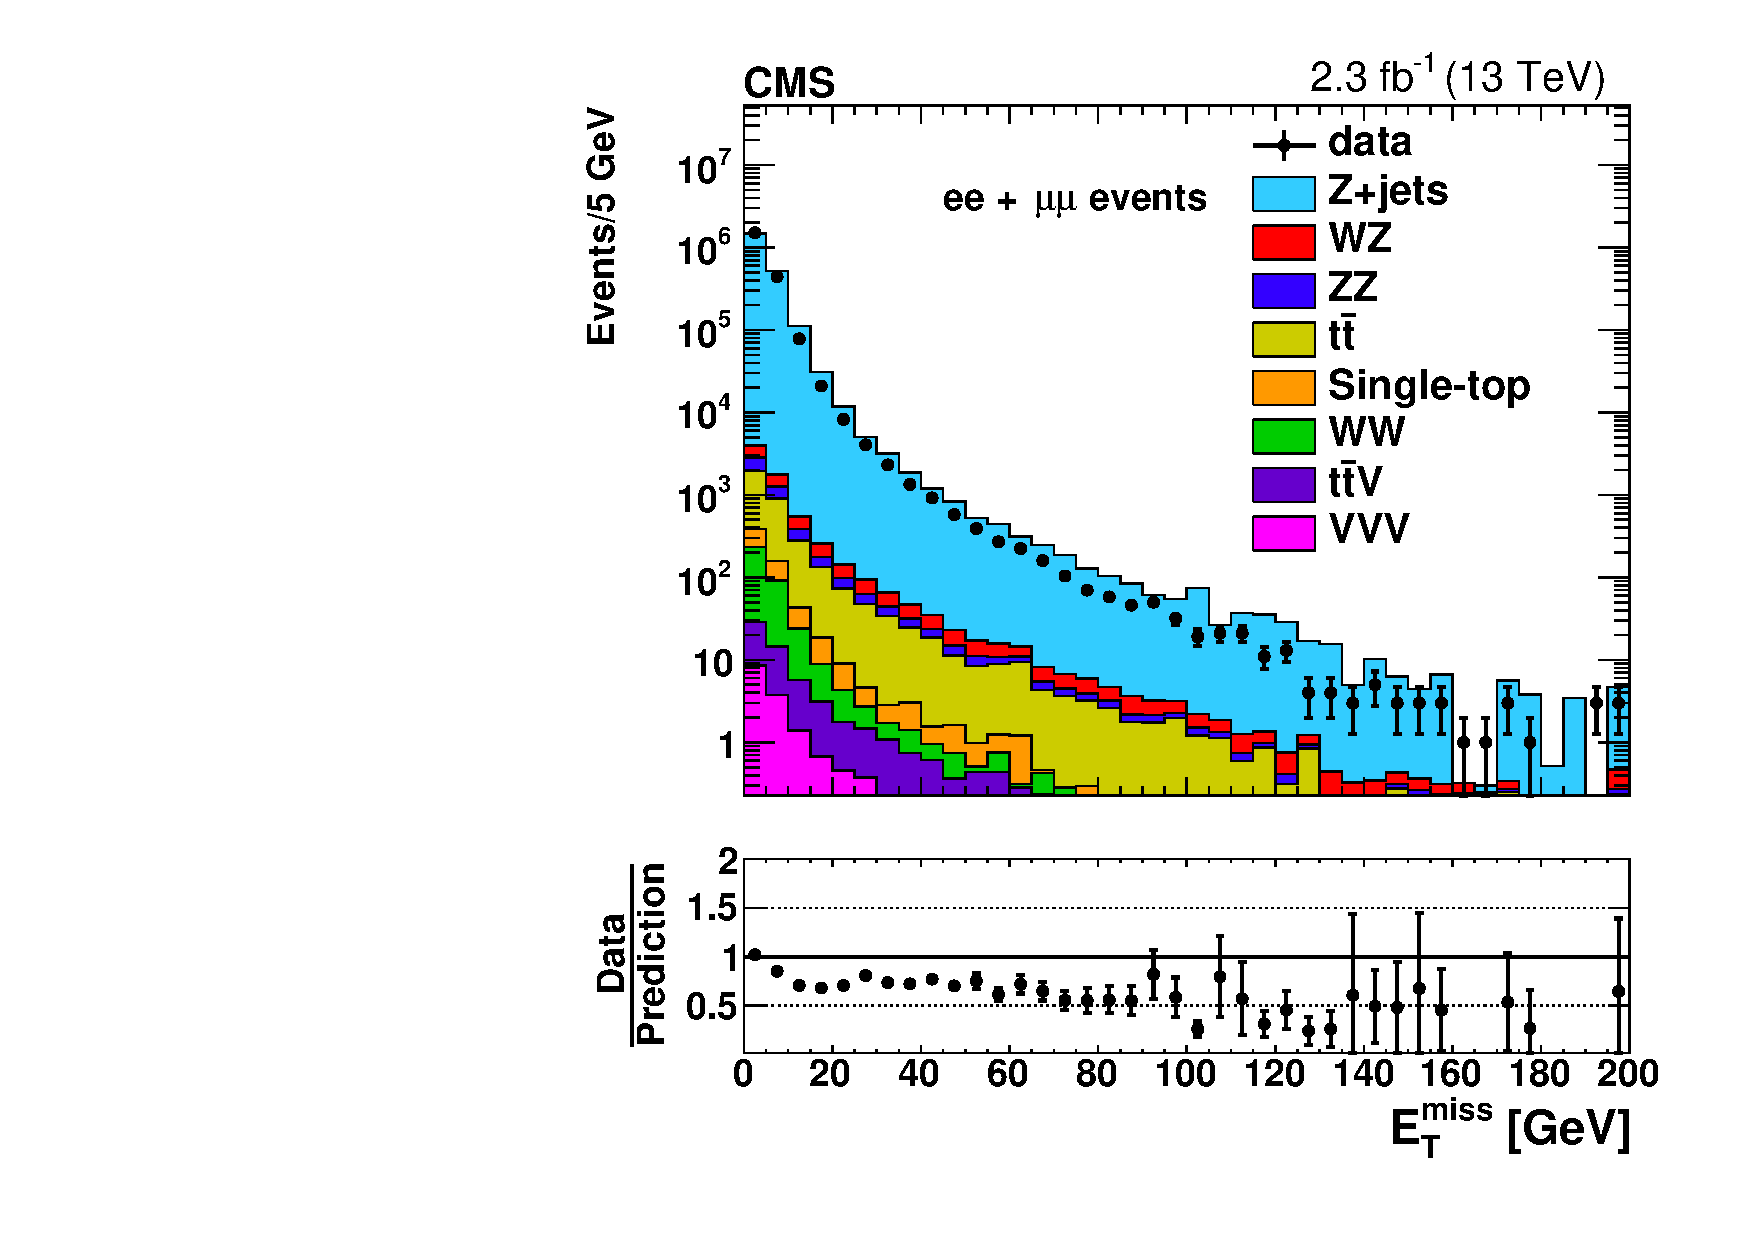
\includegraphics[width=0.4\textwidth]{MET/figs/h_met_phpfcands_2430_pt_ll_signalregion_inclusive_passtrig.pdf} \\
    \end{tabular}
    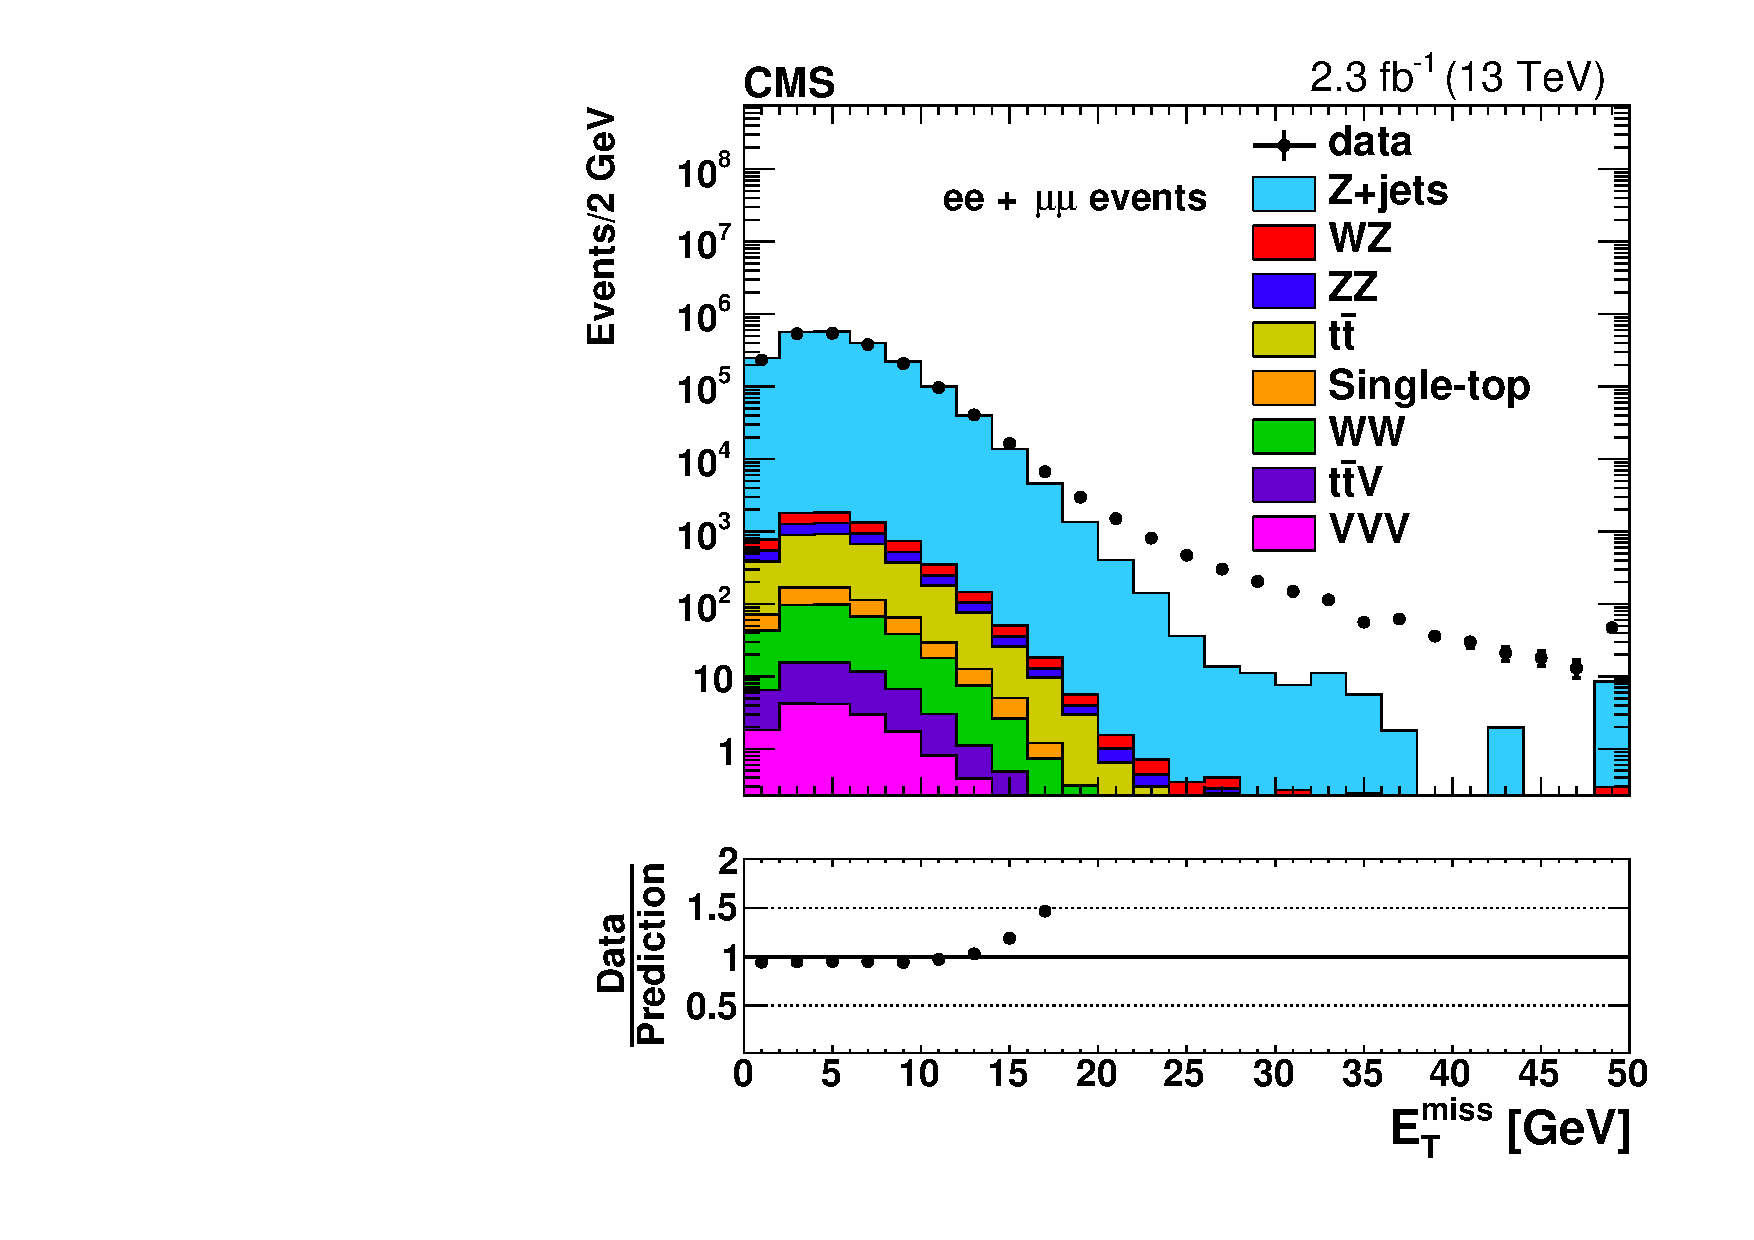
\includegraphics[width=0.4\textwidth]{MET/figs/h_met_phpfcands_30in_pt_ll_signalregion_inclusive_passtrig.pdf} 
    \caption{The \MET\ distribution is shown for neutral electromagnetic PF candidates only.
      The top row shows the barrel region on the left and transition region between the barrel and endcap on the right,
      the second row shows the endcap region including the tracker on the left and endcap region excluding the tracker on the right
      and the bottom row shows the HF region only.
      \label{fig:phpfcands}
    }
  \end{center}
\end{figure}

\begin{figure}[!htb]
  \begin{center}
    \begin{tabular}{cc}
      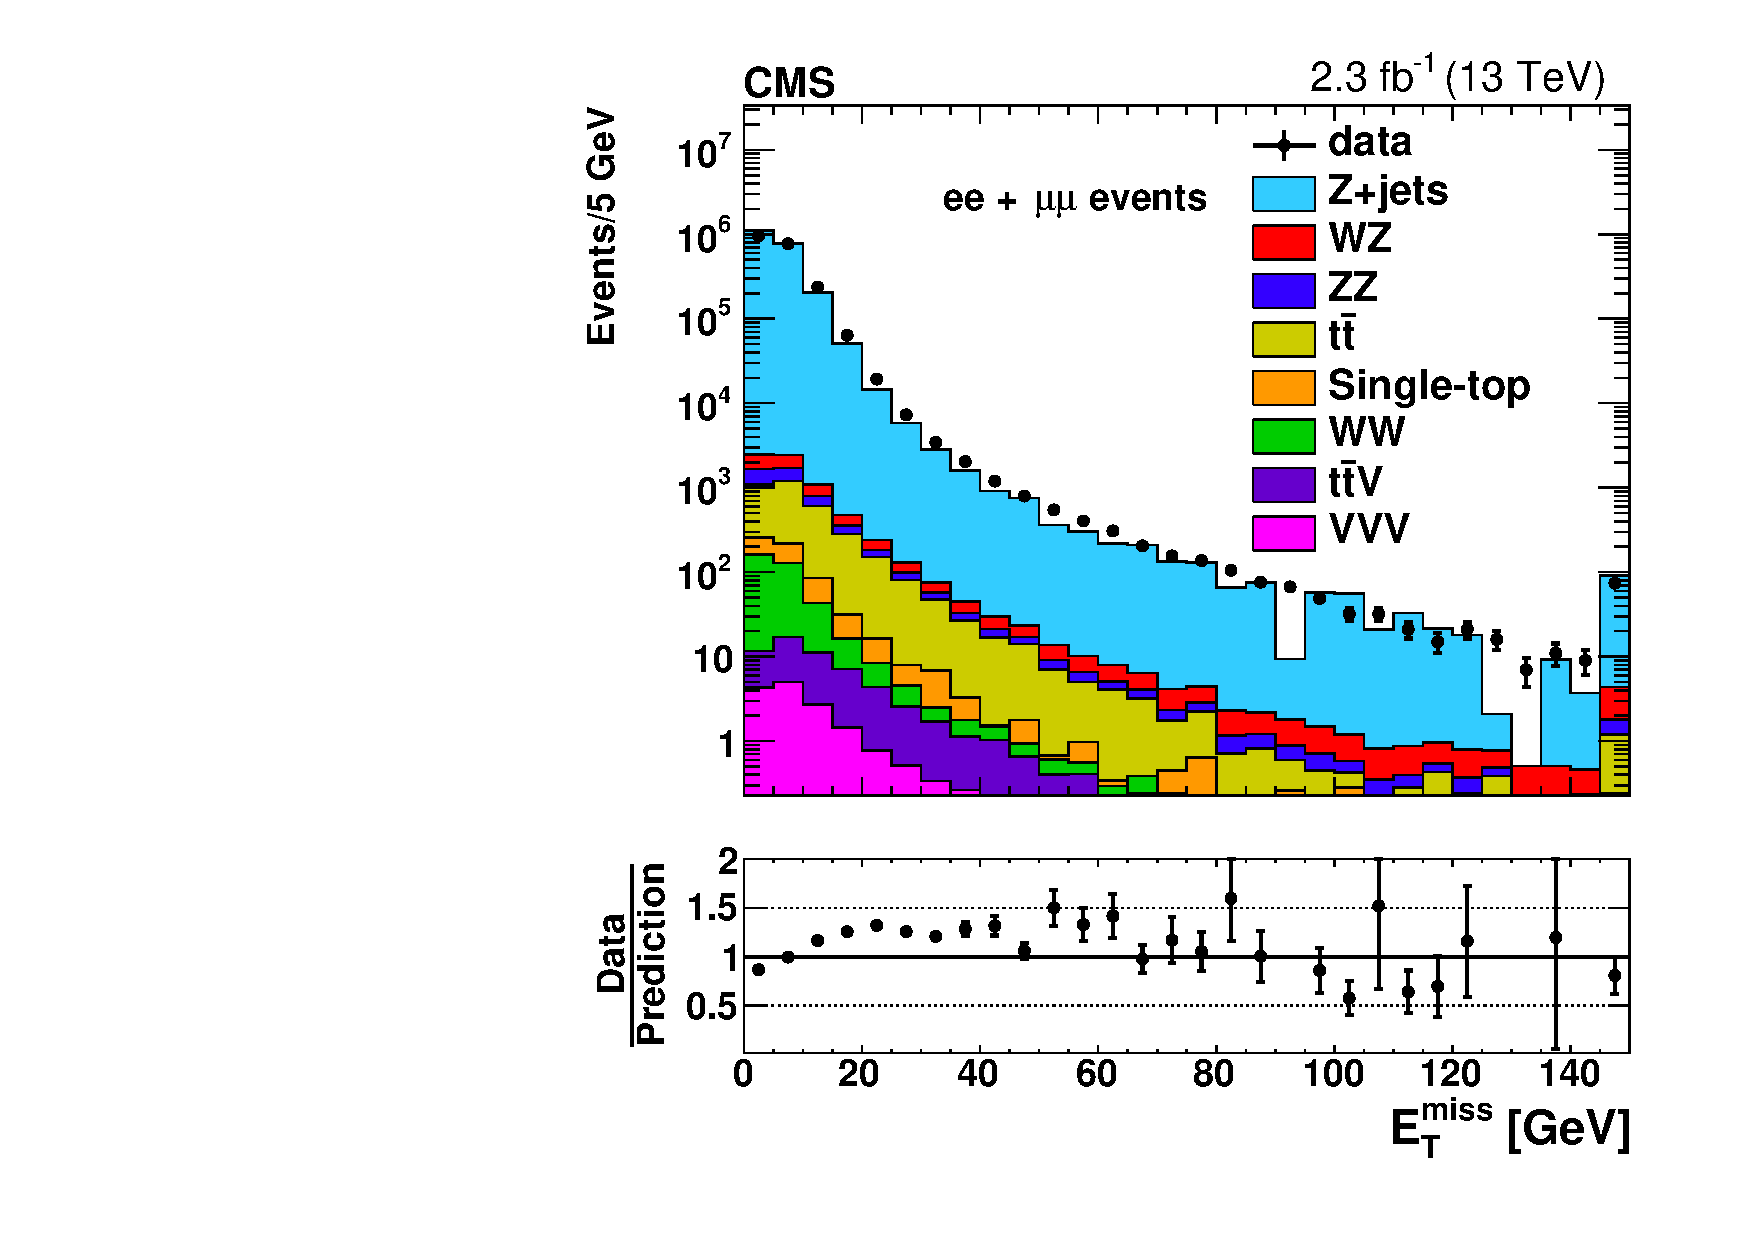
\includegraphics[width=0.4\textwidth]{MET/figs/h_met_nupfcands_0013_pt_ll_signalregion_inclusive_passtrig.pdf} &
      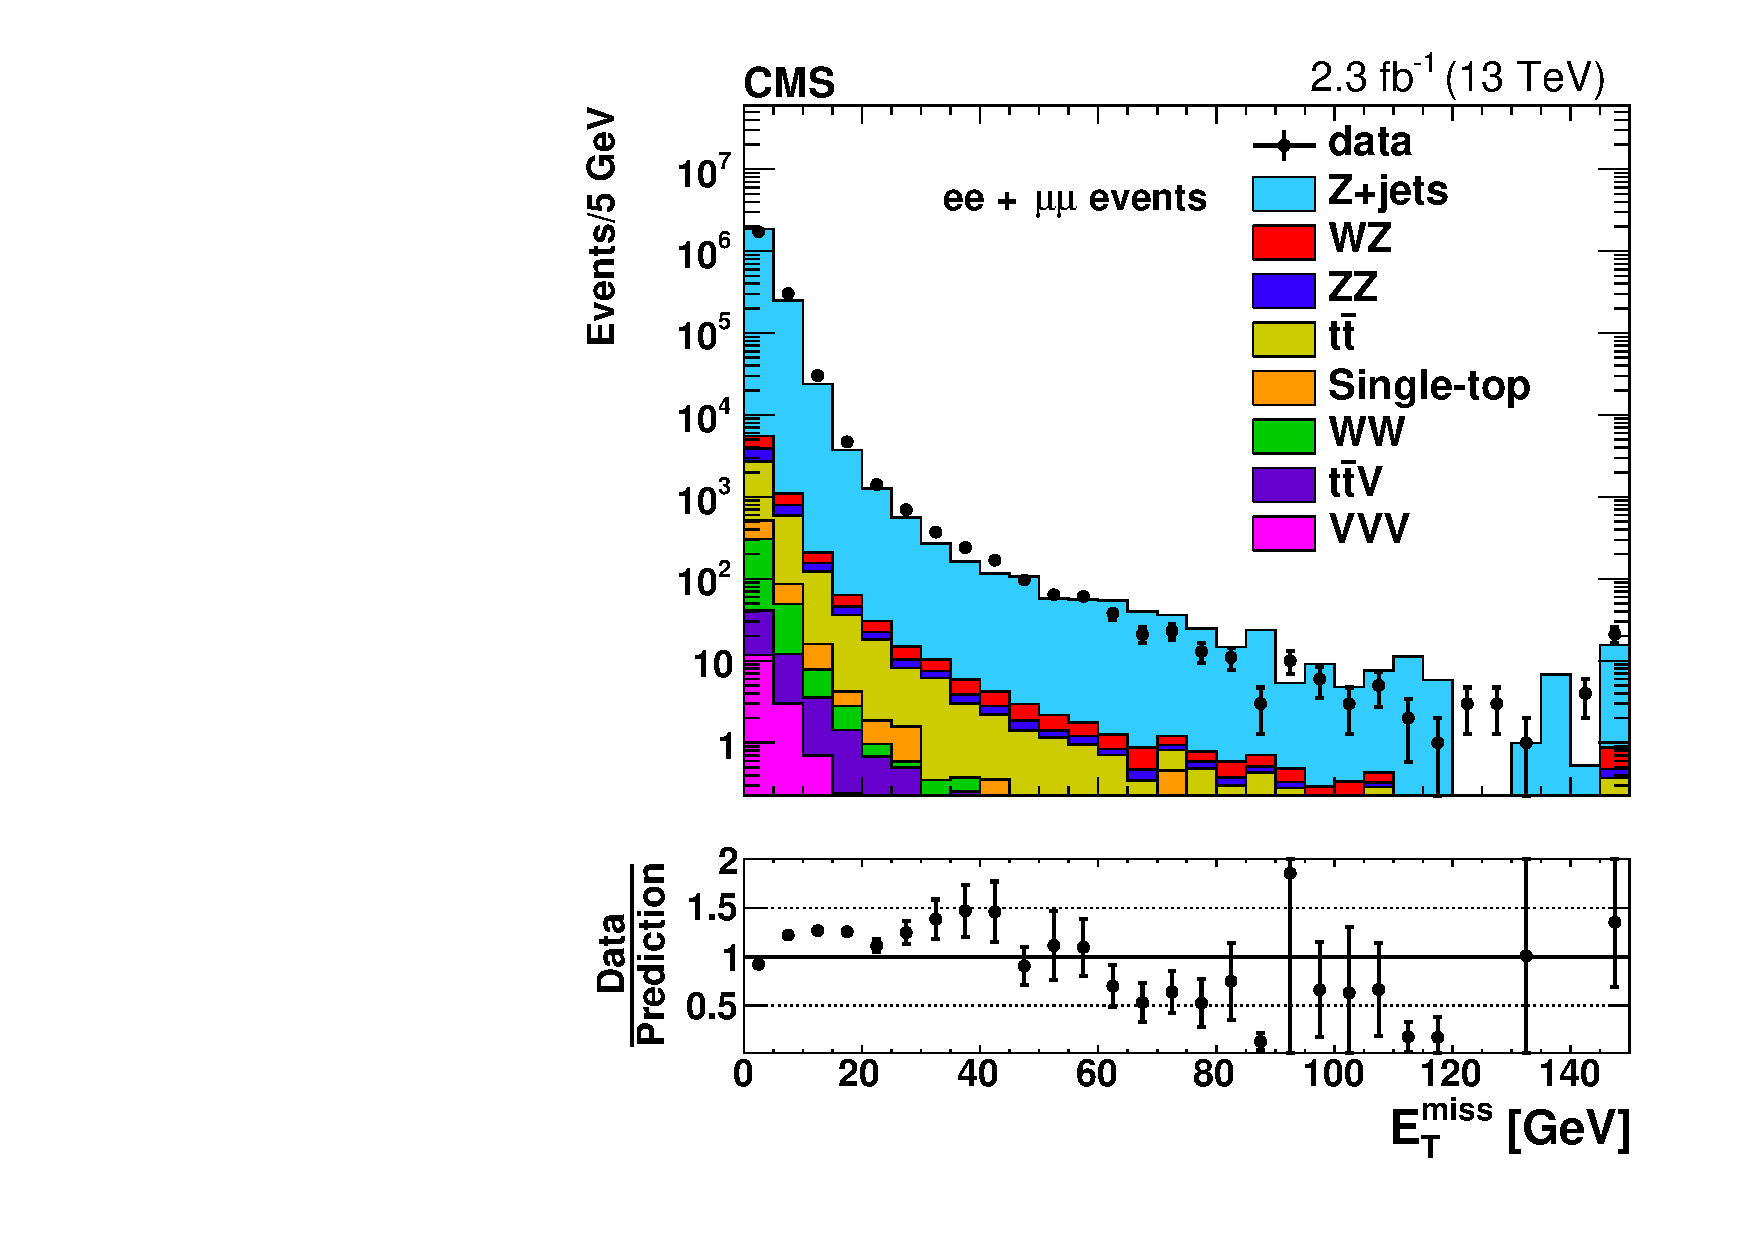
\includegraphics[width=0.4\textwidth]{MET/figs/h_met_nupfcands_1316_pt_ll_signalregion_inclusive_passtrig.pdf} \\
      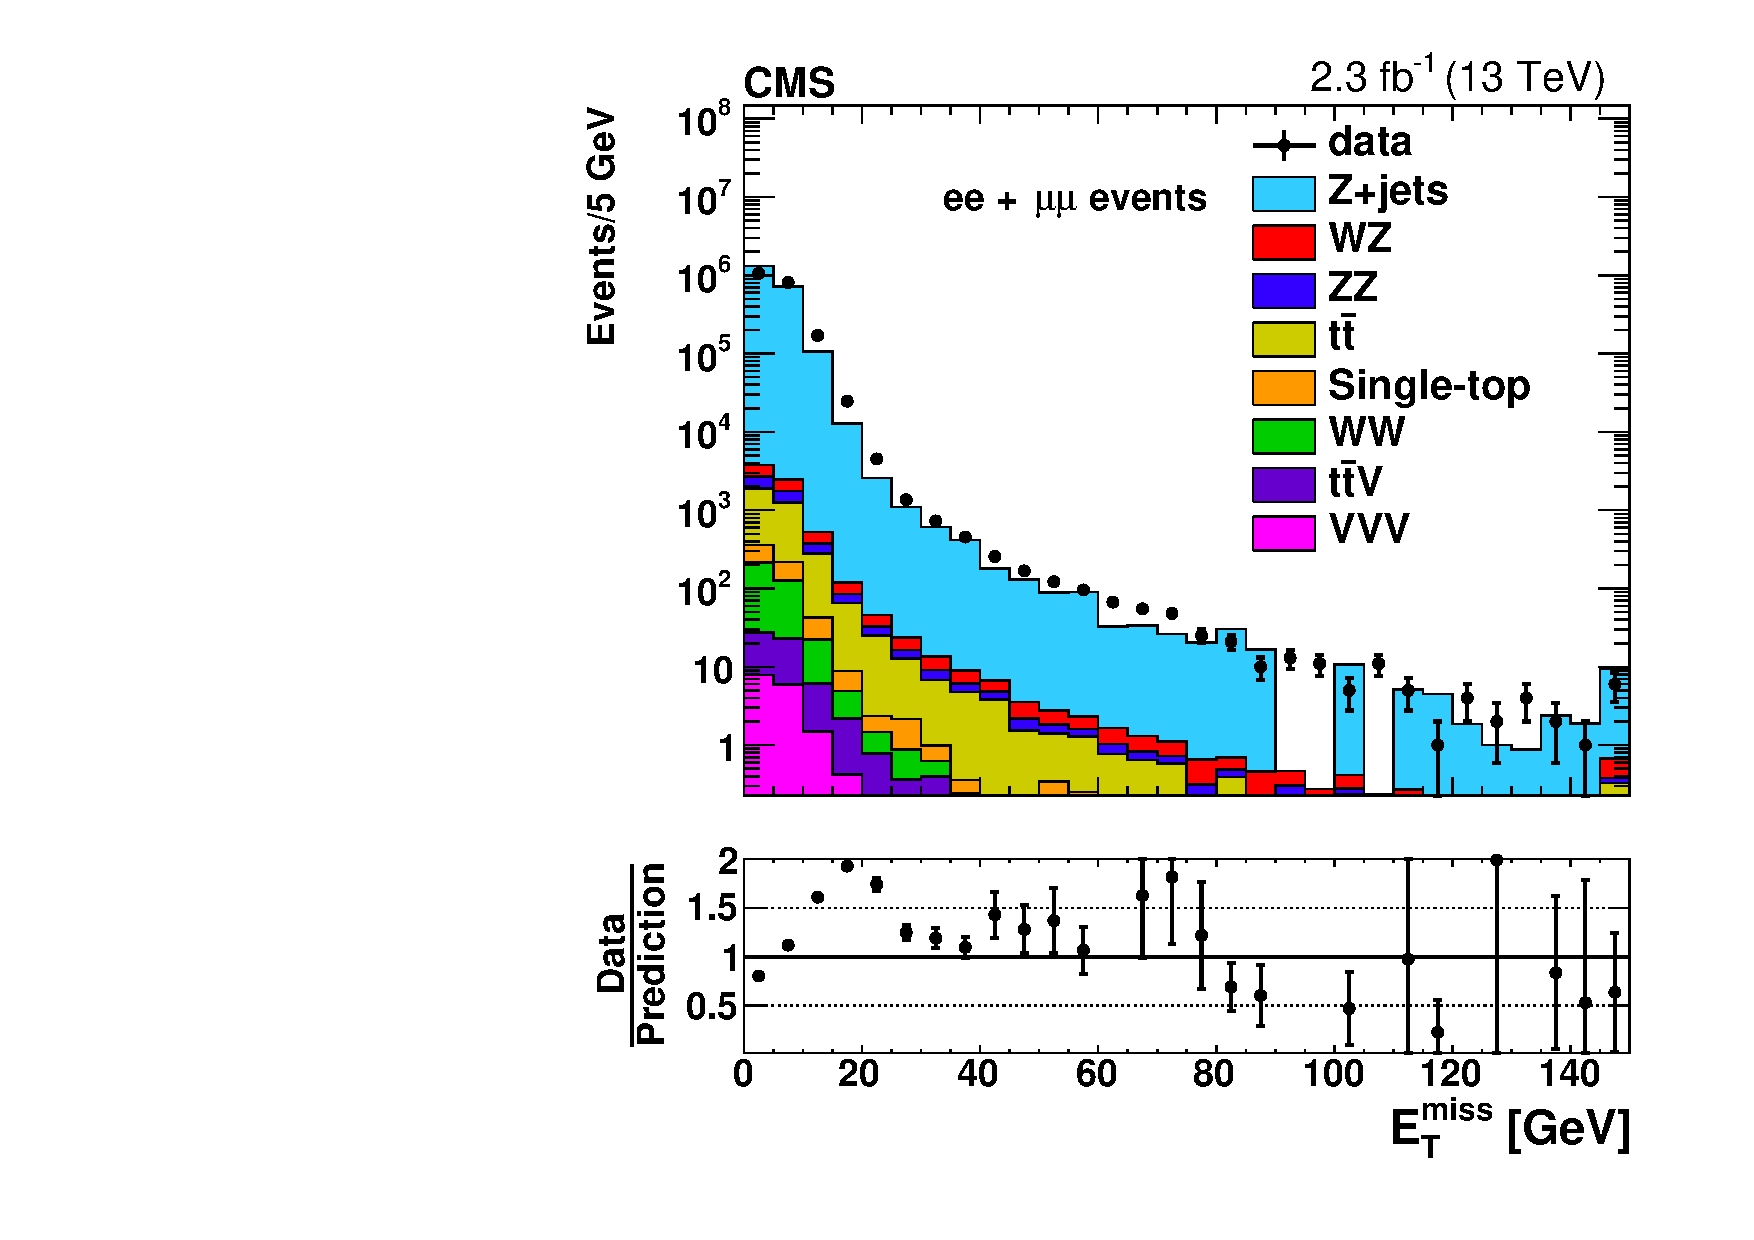
\includegraphics[width=0.4\textwidth]{MET/figs/h_met_nupfcands_1624_pt_ll_signalregion_inclusive_passtrig.pdf} &
      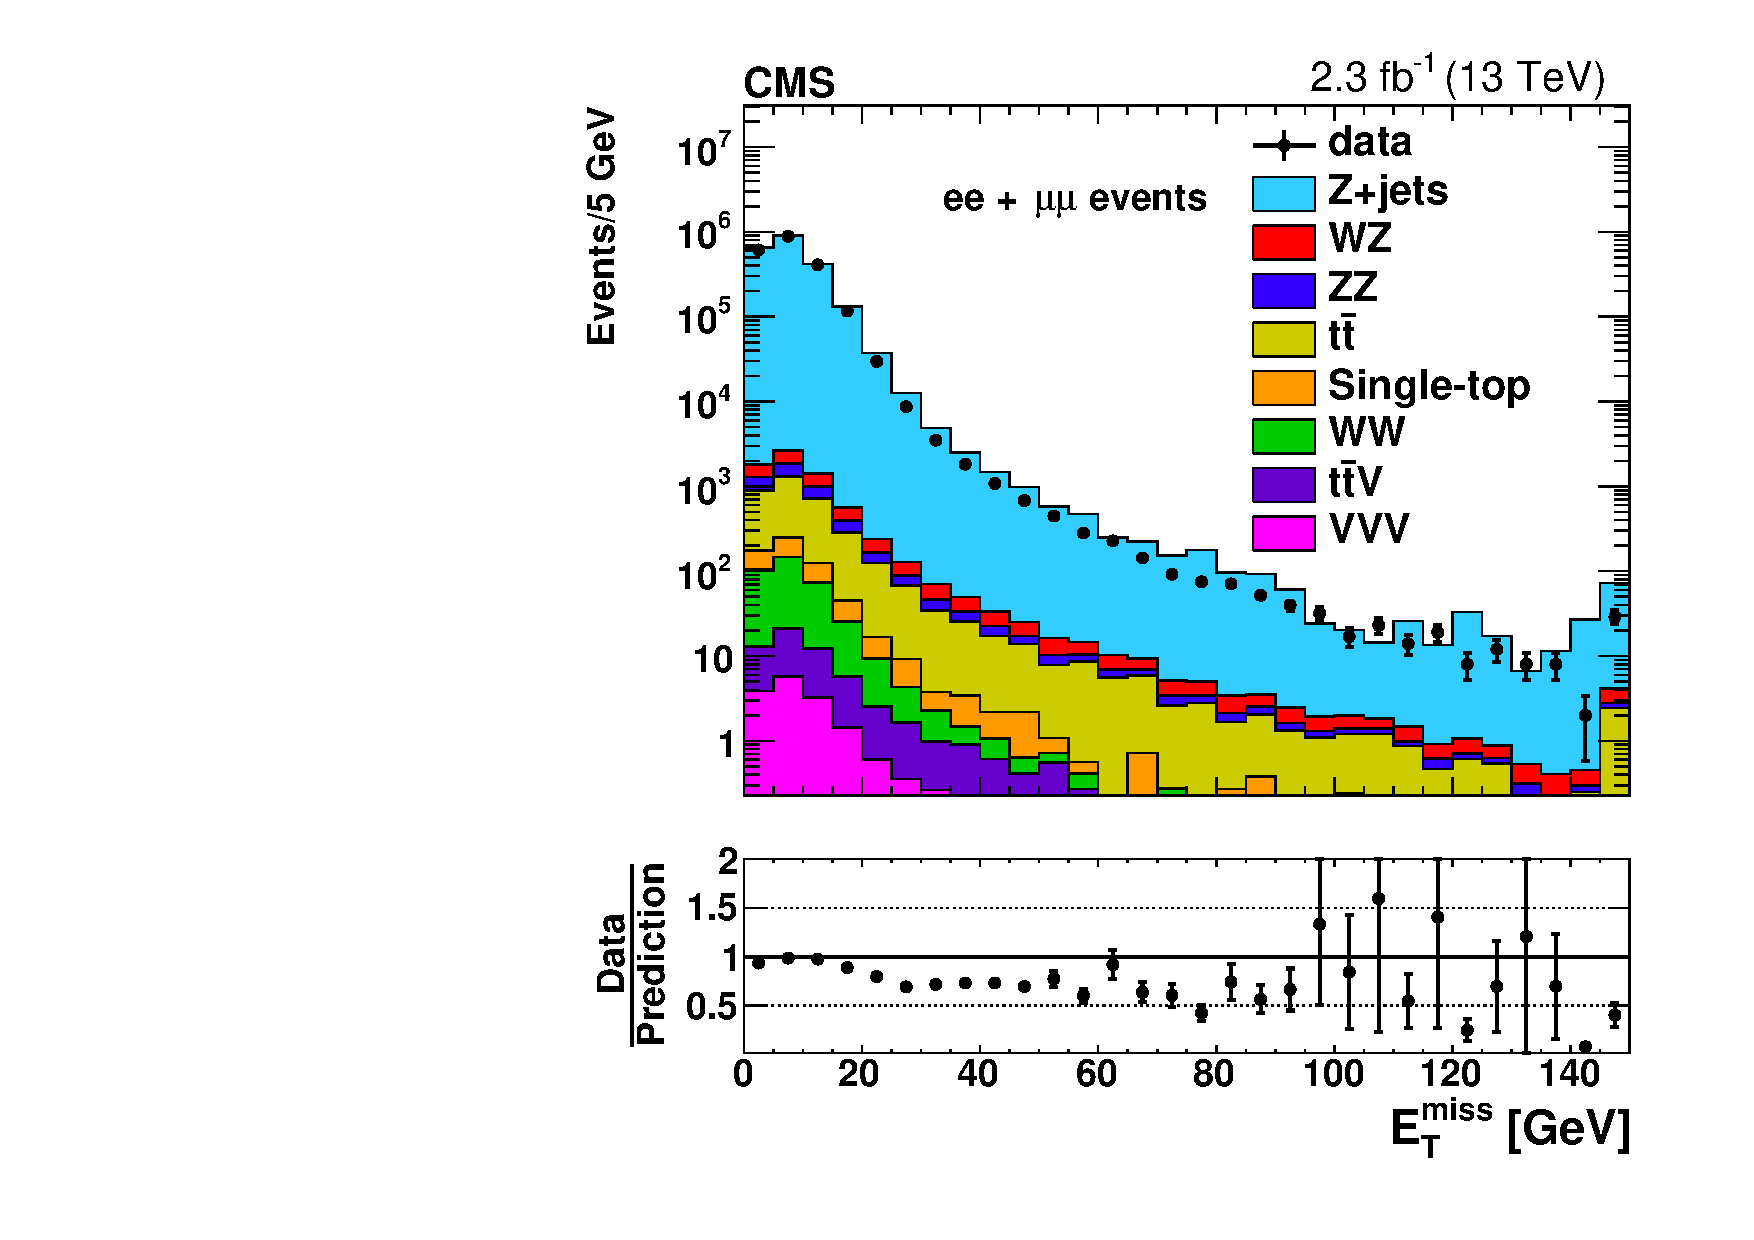
\includegraphics[width=0.4\textwidth]{MET/figs/h_met_nupfcands_2430_pt_ll_signalregion_inclusive_passtrig.pdf} \\
    \end{tabular}
    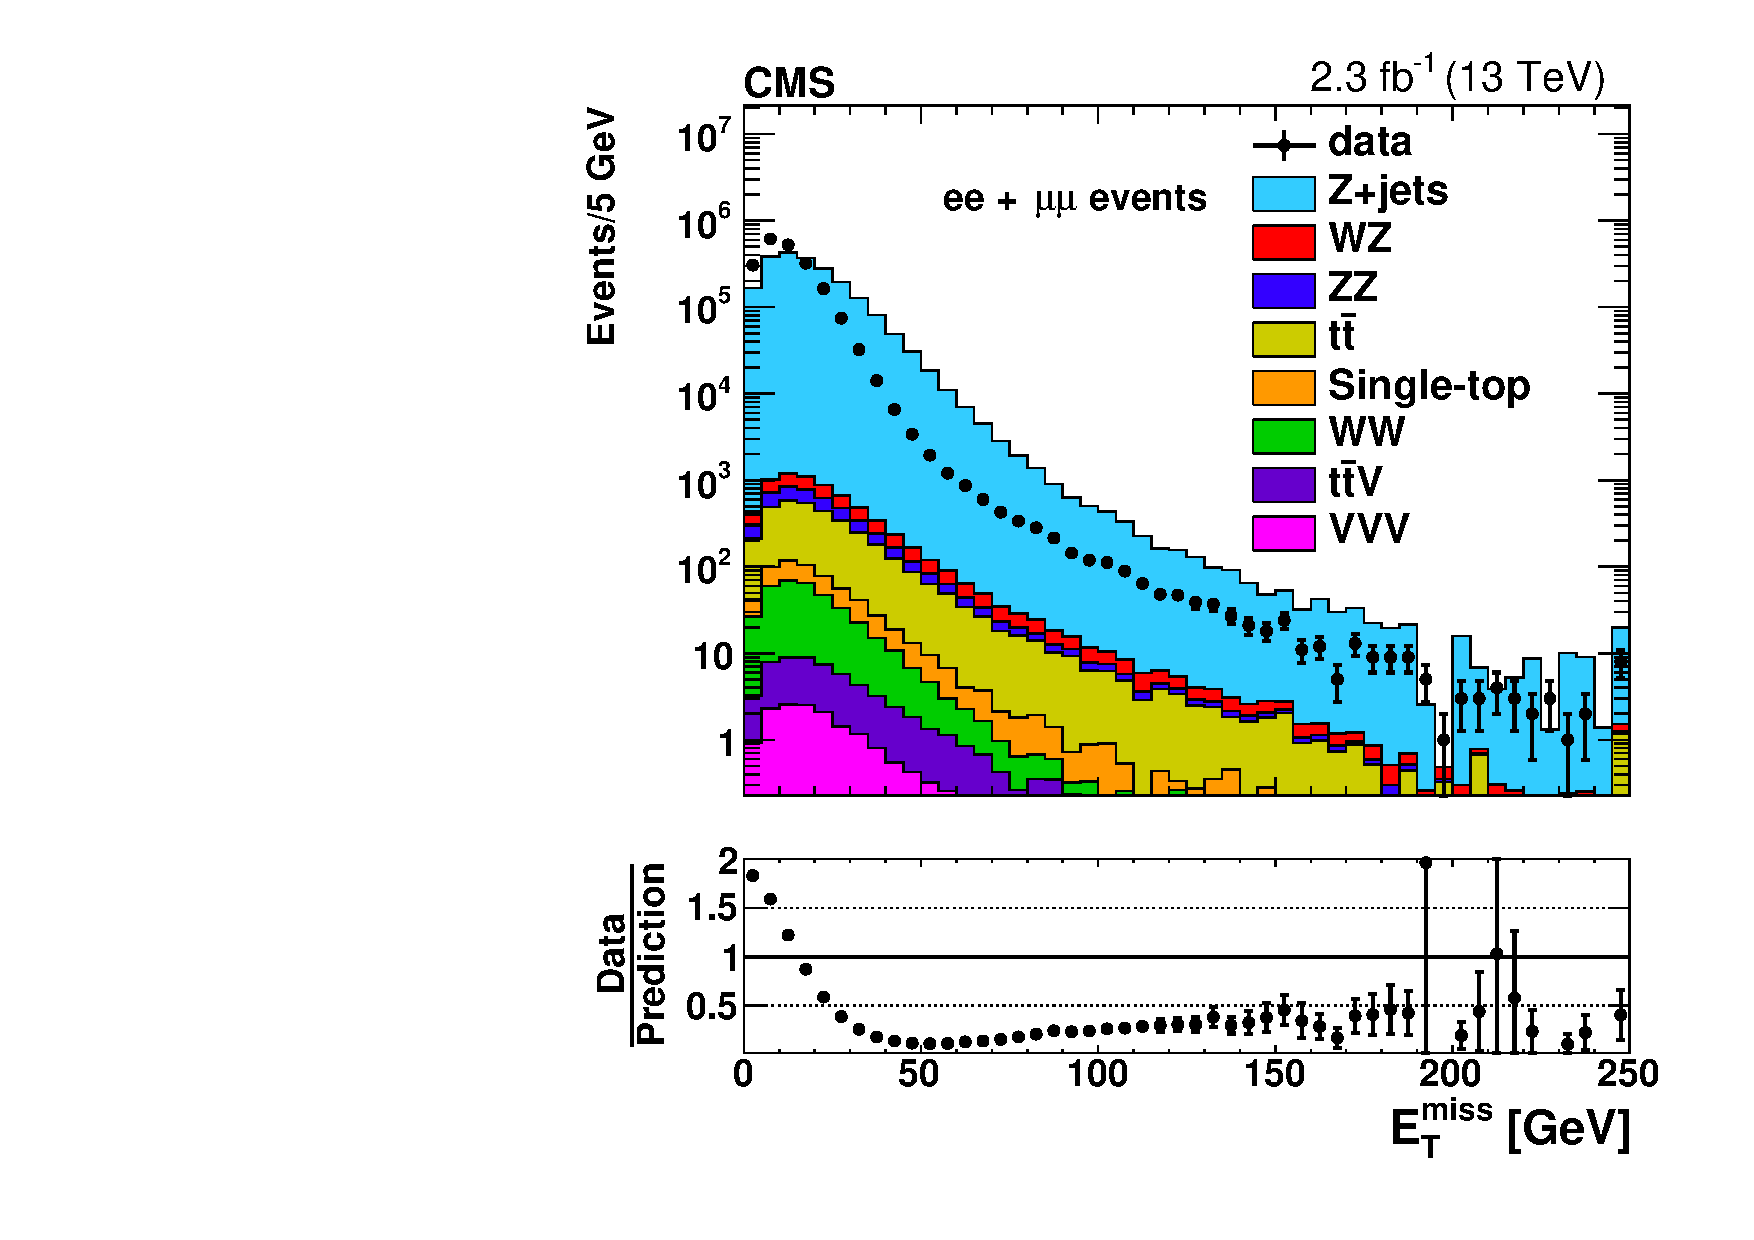
\includegraphics[width=0.4\textwidth]{MET/figs/h_met_nupfcands_30in_pt_ll_signalregion_inclusive_passtrig.pdf} 
    \caption{
      \label{fig:nupfcands}
      The \MET\ distribution is shown for neutral hadronic PF candidates only.
      The top row shows the barrel region on the left and transition region between the barrel and endcap on the right,
      the second row shows the endcap region including the tracker on the left and endcap region excluding the tracker on the right
      and the bottom row shows the HF region only.
    }
  \end{center}
\end{figure}

\clearpage

Finally, the \MET\ distribution is shown after applying the Type-1 corrections as seen in figure~\ref{fig:T1MET_datavsmc}.
Two regions are considered in order to study events with real \MET\ (\MET\ $> 100$ GeV),
and events with fake \MET\ (\MET\ $< 100$ GeV). 
Good agreement is seen in the real \MET\ region,
and reasonable agreement is seen in the fake \MET\ region.

\begin{figure}[!ht]
\begin{center}
\begin{tabular}{cc}
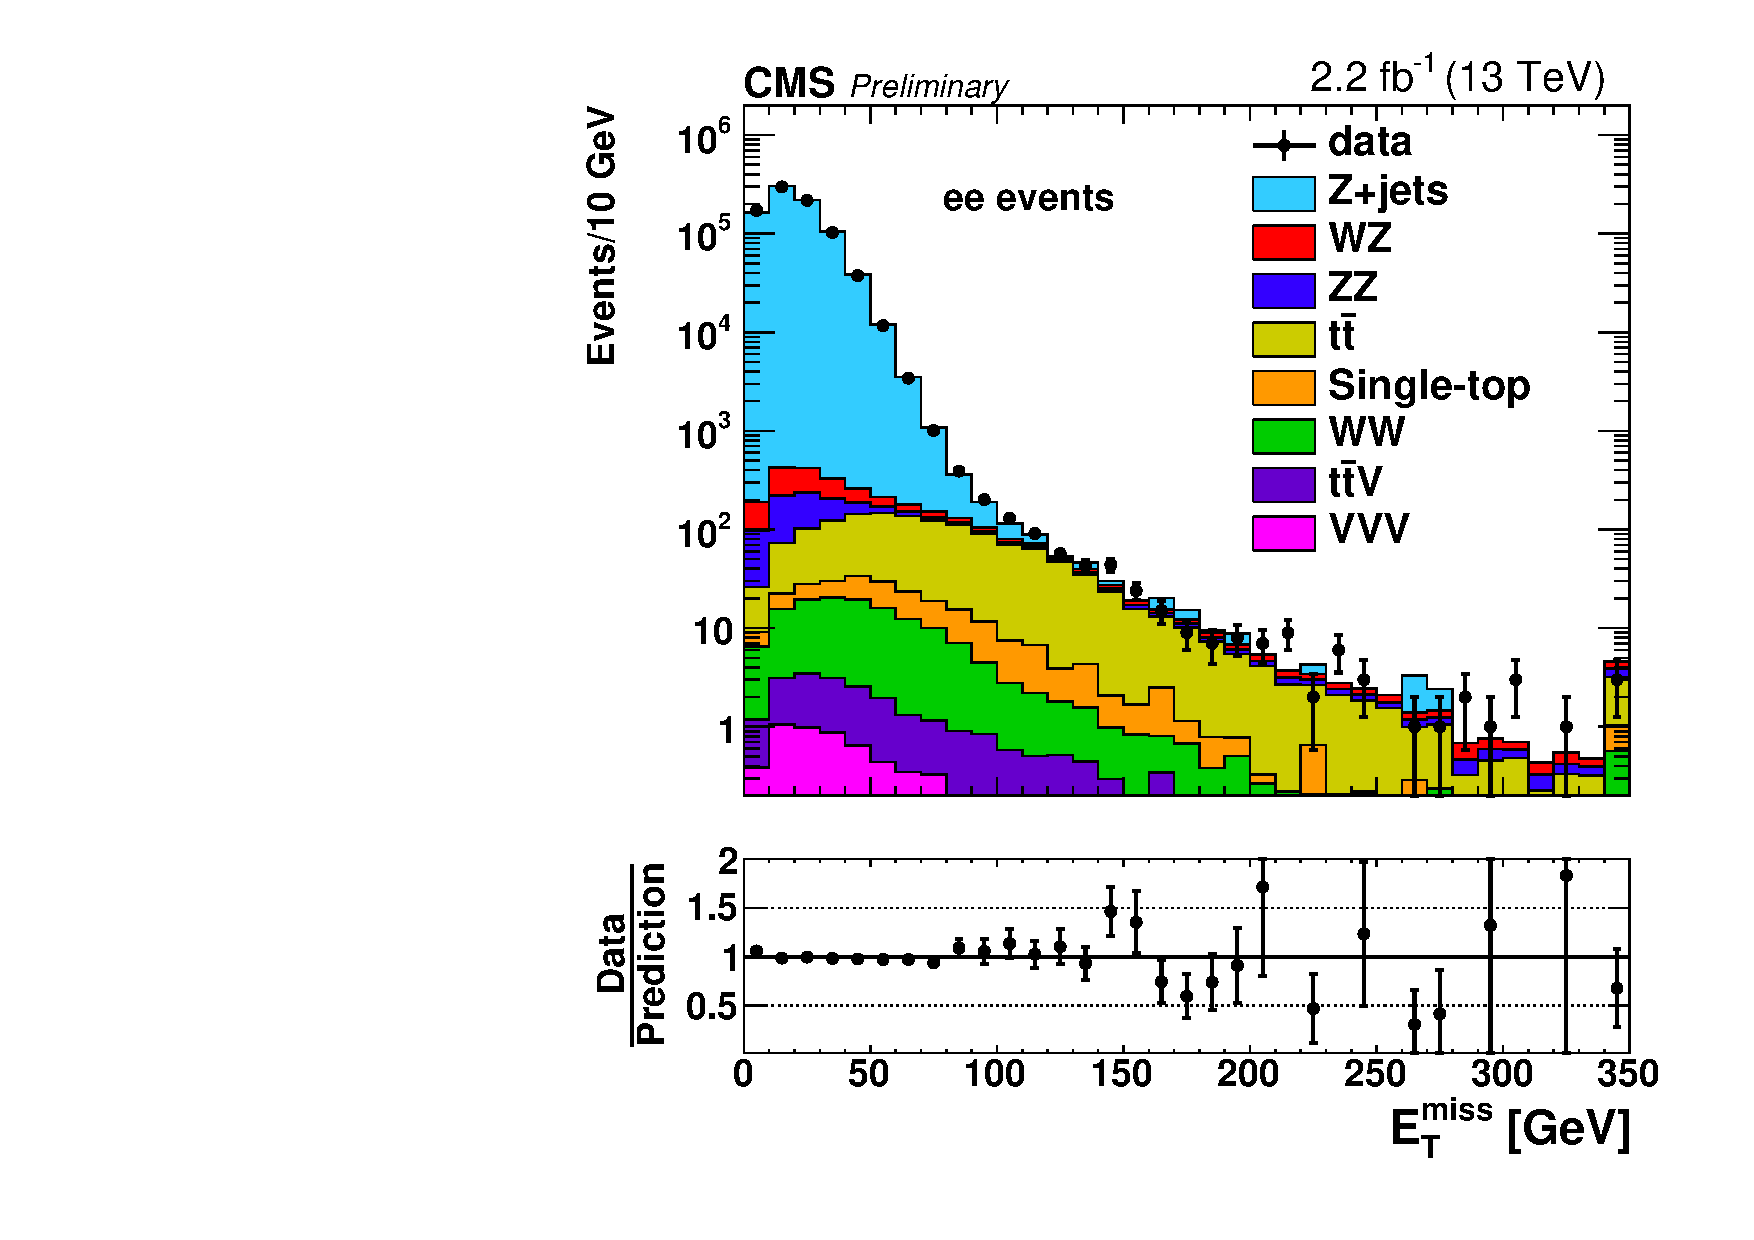
\includegraphics[width=0.4\textwidth]{MET/figs/h_met_T1CHS_pt_ee_inclusive_passtrig.pdf} &
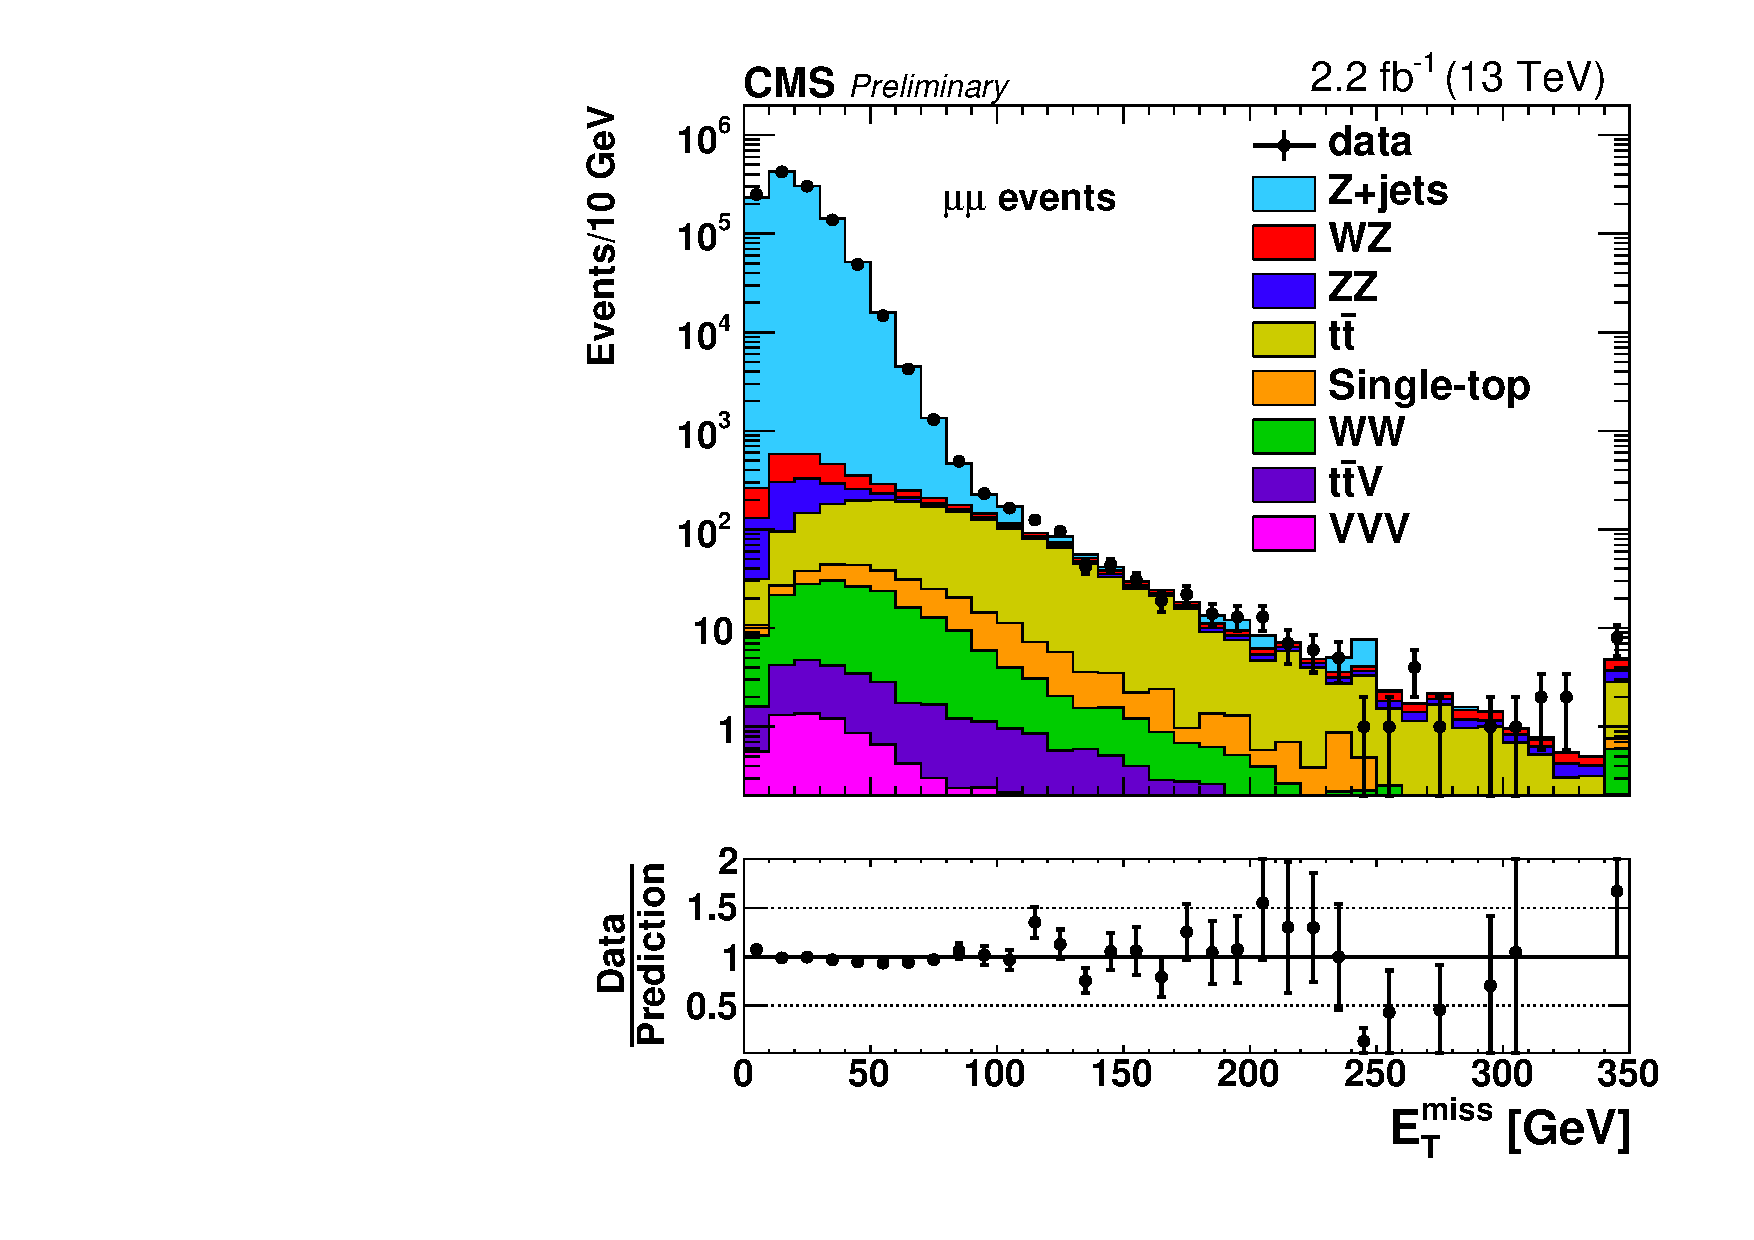
\includegraphics[width=0.4\textwidth]{MET/figs/h_met_T1CHS_pt_mm_inclusive_passtrig.pdf} \\
\end{tabular}
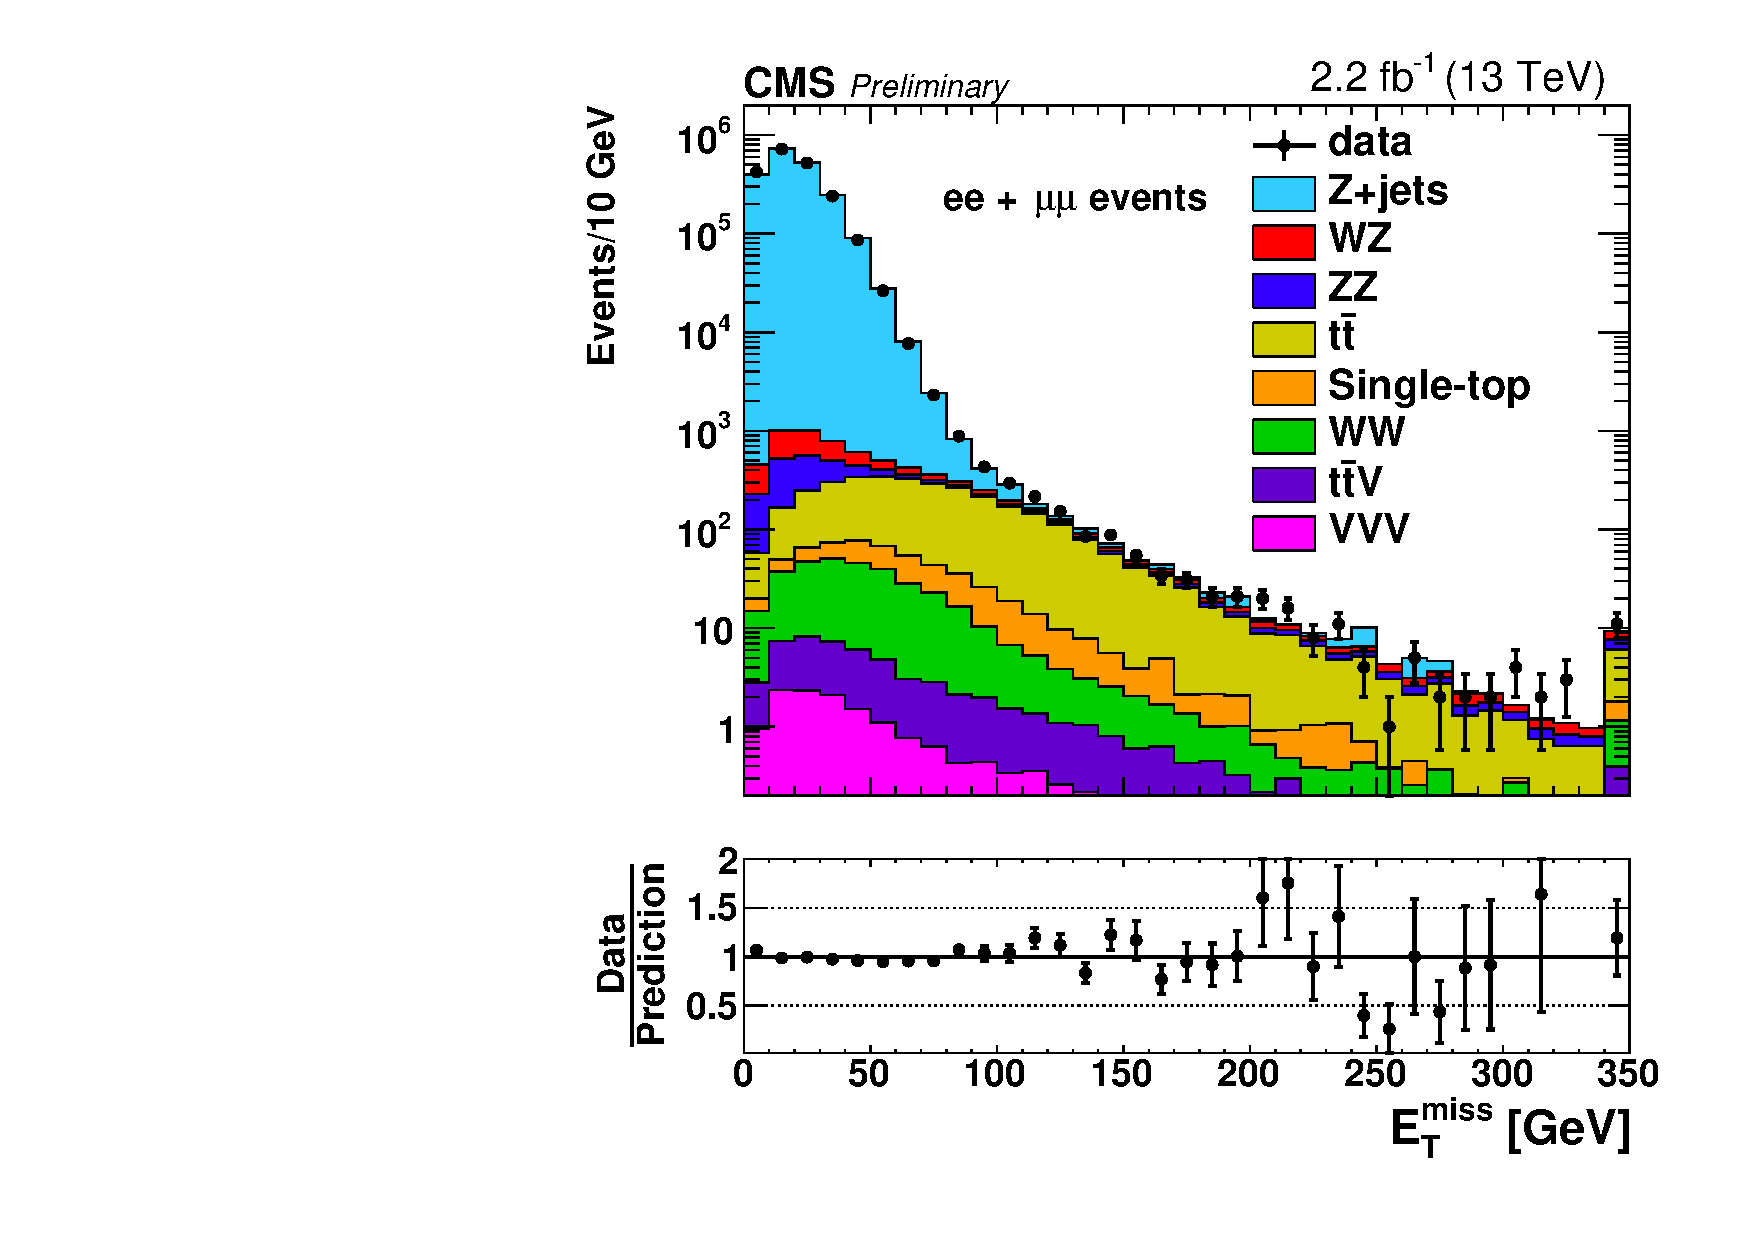
\includegraphics[width=0.6\textwidth]{MET/figs/h_met_T1CHS_pt_ll_inclusive_passtrig.pdf}
\caption{
  The \MET\ distribution is shown with data vs. MC for events while only requirement two leptons with $|M_{\ell\ell}-M_{Z}| < 10 GeV$.
  The top row shows ee events on the left and $\mu\mu$ events on the left,
  and the bottom row shows ee$+\mu\mu$ events together.
  The MC is normalized to data.
\label{fig:T1MET_datavsmc}
}
\end{center}
\end{figure}

\subsection{Data-driven \texorpdfstring{\MET}{MET}\ Predictions}
Although good agreement is seen in data and MC after applying Type-1 corrections to \MET, 
it's clear that there are still problems with the simulation based on the studies in section~\ref{subs:MET_datavsmc}.
Additionally, a new discovery in physics is important enough that it is imperatave that the background predictions can be trusted.
Therefore, it's important to make sure there is a reliable prediction for backgrounds coming from standard model processes in regions with large values of \MET.
Techniques were developed to predict the largest backgrounds using control regions in data,
and these techniques are described in detail in chapter~\ref{ch:bkgd}.
